\documentclass[parskip=half]{scrreprt}
\usepackage[utf8]{inputenc}
\usepackage[T2A, T1]{fontenc}
\usepackage[ngerman]{babel}
\usepackage{amsmath}
\usepackage{amsfonts}
\usepackage{amssymb}
\usepackage{geometry}
\usepackage{environ}
\usepackage[inline]{enumitem}
\usepackage[many]{tcolorbox}
\usepackage{siunitx}
\usepackage{trfsigns}
\usepackage{todonotes}
\usepackage{graphics}
\graphicspath{{Bilder/}}
\sisetup{locale=DE}


% Title Page
\title{Signale und Systeme Boxen}
\author{Florian Lubitz \& Steffen Hecht}

\newcounter{BoxCounter}
\setcounter{BoxCounter}{0}


\newtcolorbox{dbox}[1][]{%
	enhanced,frame hidden,interior hidden,
	arc=0pt,outer arc=0pt,borderline={0.4pt}{0pt}{dashed},
	nobeforeafter, box align=center, before={\stepcounter{BoxCounter}\boxed{\arabic{BoxCounter}}\makebox[.5cm]{}}, 
	after={\vspace{0.5cm}}, #1
}

\NewEnviron{tbox}{%
	\begin{dbox}[width=\textwidth]
		\BODY
	\end{dbox}
}
\NewEnviron{abox}{%
	\begin{dbox}[width=\textwidth]	
		\begin{align*}
		\BODY
		\end{align*}
	\end{dbox}
}
\makeatletter
\newcommand{\numbereq}{%
	\ifmeasuring@
	\else
	\refstepcounter{equation}%
	\fi
	\tag{\theequation}%
}

% Kyrillische Buchstaben
\newcommand{\KW}{\mbox{\usefont{T2A}{\rmdefault}{m}{n}\CYRSHCH}}


\newcommand*{\rom}[1]{\expandafter\@slowromancap\romannumeral #1@}

\newcommand{\ztrans}{\rotatebox[origin=c]{-90}{$\laplace$}}
\newcommand{\ztransrueck}{\rotatebox[origin=c]{90}{$\laplace$}}
\newcommand{\rect}{\text{rect}}
\newcommand{\ramp}{\text{ramp}}
\newcommand{\sramp}{\text{sramp}}
\newcommand{\tri}{\text{tri}}
\newcommand{\sLaplace}{\text{ }\Laplace\text{ }}
\newcommand{\slaplace}{\text{ }\laplace\text{ }}

\makeatother

\begin{document}
	\maketitle

	% Comment parts out to speed up compile times

	% !TeX root = ../SigSysBoxen.tex

	\chapter{Motivation, Wiederholung und Überblick}
\begin{tbox}
	a
\end{tbox}

\begin{abox}
	\underline{U}_1 &= U_1 \angle \varphi_1 = \frac{30}{\sqrt{2}} \angle \frac{\pi}{3}\\
	\underline{Z}_R &= R = 1000\\
	\underline{Z}_C &= \frac{1}{j \omega C} = \frac{1}{sC} = \frac{1000}{s}
\end{abox}

\begin{abox}
	H(s) := \frac{\underline{U}_2}{\underline{U}_1} = \frac{\underline{Z}_C}{\underline{Z}_R + \underline{Z}_C} = \frac{\frac{1}{sC}}{R + \frac{1}{sC}} = \frac{1}{1 + sRC} = \frac{1}{1 + s}
\end{abox}

\begin{abox}
	\left|H(j\omega)\right| &= \left|\frac{1}{1 + j\omega RC}\right| = \frac{1}{\left|1 + j\omega RC\right|} = \frac{1}{\sqrt{1^2 + (\omega RC)^2}} = \frac{1}{\sqrt{1 + \omega^2}}\\
	\sphericalangle H(j\omega) &= \sphericalangle \frac{1}{1 + j\omega RC} = \sphericalangle \frac{1 - j \omega RC}{1 + (\omega RC)^2} = \arctan\left(\frac{\frac{-\omega RC}{1 + (\omega RC)^2}}{\frac{1}{1 + (\omega RC)^2}}\right)\\
	&= \arctan(\omega RC) = -\arctan(\omega)\\
	\underline{U}_2 &= H(s) \cdot \underline{U}_1 = \left|H(j\omega)\right| \cdot \left|\underline{U}_1\right| \angle\varphi_1 \sphericalangle H(j\omega)\\
	&= \frac{1}{\sqrt{1 + \omega^2}} \cdot \left|\underline{U}_1\right| \angle (\frac{\pi}{3} - \arctan(\omega))
\end{abox}

\begin{abox}
	a) \quad\underline{U}_2 &= \frac{1}{\sqrt{1 + (2\pi \cdot 0,5)^2}} \cdot 21.2 \angle \frac{\pi}{3} - \arctan(2\pi \cdot 0,5) \approx 6,43\angle -0,21\\
	&\Rightarrow u_2(t) = 6,43 \cdot\sqrt{2} \cdot \sin(2\pi \cdot 0,5 \cdot t - 0,21) \approx \SI{9,09}{\volt} \cdot \sin(\pi t - 0,21)\\
	b) \quad\underline{U}_2 &\approx 0,67\angle -0,49 \Rightarrow u_2(t) \approx \SI{0,95}{\volt} \cdot \sin(10\pi t - 0,49)\\
	c) \quad\underline{U}_2 &\approx 0,0067\angle -0,523 \Rightarrow u_2(t) \approx \SI{9,55}{\milli\volt} \cdot \sin(100\pi t - 0,523)
\end{abox}

\begin{abox}
	&\text{Für}\quad x(t) = \SI{30}{\volt}\sin(\pi t + \pi / 3)\quad \text{ist}\quad \mathcal{H}\{x(t)\} = \SI{9,09}{\volt}\sin(\pi t - 0,21)\\
	&\text{Für}\quad y(t) = \SI{30}{\volt}\sin(10\pi t + \pi / 3)\quad \text{ist}\quad \mathcal{H}\{y(t)\} = \SI{0,95}{\volt}\sin(10\pi t - 0,49)
\end{abox}

\begin{tbox}
	\begin{align*}
	u_1(t) = \SI{15}{\volt}\sin(\pi t + \pi/3) + \SI{60}{\volt}\sin(10\pi t + \pi/3) = 0,5x(t) + 2y(t)
	\end{align*}
	und damit $a = 0,5, b=2$ und
	\begin{align*}
	u_2(t):= \mathcal{H}\{u_1(t)\} = \mathcal{H}\{0,5x(t) + 2y(t)\} \overset{??}{=}
	\end{align*}
\end{tbox}

\begin{abox}
	&\mathcal{H}\{ax(t) + by(t) + cz(t)\} = \mathcal{H}\{ax(t) + 1 \cdot (by(t) + cz(t)\}\\
	&\overset{(??)}{=} a\mathcal{H}\{x(t)\} + 1 \cdot \mathcal{H}\{by(t) + cz(t)\} \overset{(??)}{=} a\mathcal{H}\{x(t)\} + b\mathcal{H}\{y(t)\} + c\mathcal{H}\{z(t)\}
\end{abox}

\begin{abox}
	x[-\infty],\dots,x[-3],x[-2],x[-1],x[0],x[1],x[2],x[3],\dots,x[\infty]
\end{abox}

\begin{tbox}
	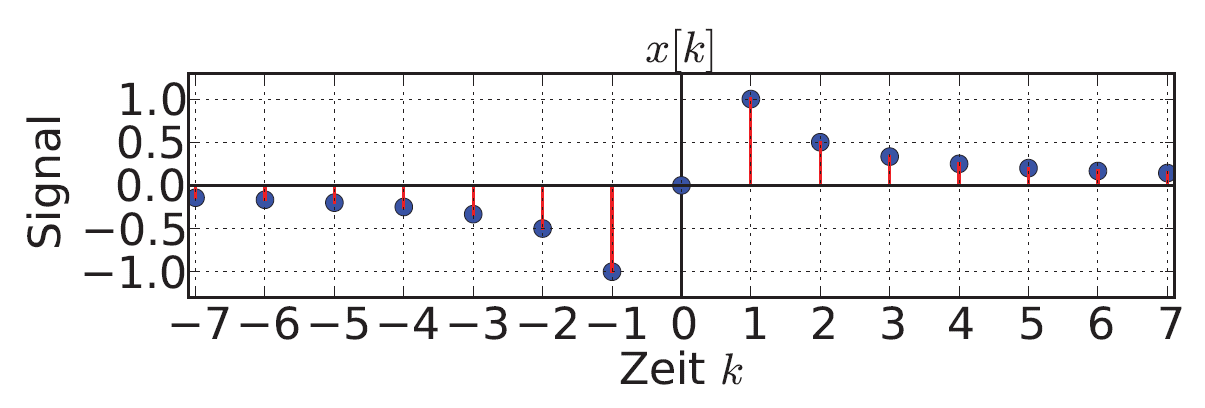
\includegraphics[width=\textwidth]{Box9}
\end{tbox}

\begin{tbox}
	\begin{itemize}
		\item $x[-k]$ die \underline{Spiegelung} von $x[k]$ an der Signalpegel-Achse
		\item  $x[k + k_0]$ die \underline{Verschiebung von $x[k]$ um $k_0$ nach links}
		\item  $x[k - k_0]$ die \underline{Verschiebung von $x[k]$ um $k_0$ nach rechts}
	\end{itemize}
\end{tbox}

\chapter{Diskrete Signale}
\setcounter{BoxCounter}{10}
\begin{tbox}
\end{tbox}

\begin{tbox}
	\begin{alignat*}{2}
	&(b) \quad x[-k] &&= \begin{cases}
	-\frac1k,\quad k \ne 0 \\
	0,\quad k = 0
	\end{cases}
	\\
	&(c)\quad  x[k+k_0] = x[k+3] &&= \begin{cases}
	\frac{1}{k+3}, \quad k \ne -3 \\
	0, \quad k = -3
	\end{cases}\\
	&(d)\quad  x[k-k_0] = x[k-3] &&= \begin{cases}
	\frac{1}{k-3}, \quad k \ne 3 \\
	0, \quad k = 3
	\end{cases}
	\end{alignat*}
\end{tbox}

\begin{abox}
	x[k_0 - k] &= x[-(k - k_0)]\\
	&= x[(-k) + k_0]
\end{abox}

\begin{abox}
	\text{mit} \quad x[k_0 -k] = x[3 - k] = \begin{cases}
		\frac{1}{3-k}, \quad k \ne 3\\0 , \quad k = 3
	\end{cases}
\end{abox}

\begin{tbox}
	\begin{itemize}
		\item $x[k]$ heißt \underline{gerades Signal}, falls $x[k] = x[-k]$ $\forall k \in \mathbb{Z}$ gilt.
		\item $x[k]$ heißt \underline{ungerades Signal}, falls $x[k] = -x[-k]$ $\forall k \in \mathbb{Z}$ gilt.
	\end{itemize}
\end{tbox}

\begin{abox}
	x[-k] = \begin{cases}
		\frac{1}{-k}, \quad k \ne 0\\
		0, \quad k = 0
	\end{cases} = \begin{cases}
		-\frac1k, \quad k \ne 0 \\ 
		0, \quad k = 0 
	\end{cases}  = -x [k] 
\end{abox}

\begin{abox}
	y[-k] = \begin{cases}
		\frac{1}{(-k)^2}, \quad k \ne 0\\
		0, \quad k = 0
	\end{cases} = \begin{cases}
		-\frac{1}{k^2}, \quad k \ne 0 \\
		0, \quad k = 0 
	\end{cases}  = y [k] 
\end{abox}

\begin{tbox}
	\begin{itemize}
		\item  $x[k]$ heißt \underline{kausales Signal}, falls gilt: $x[k] = 0$ $\forall k < 0$
		\item $x[k]$ heißt \underline{nicht-kausales Signal}, falls gilt $\exists k < 0 : x[k] \ne 0$
		\item $x[k]$ heißt \underline{anti-kausales Signal}, falls $x[-k-1]$ kausal ist, d.h. falls gilt: $x[k] = 0$ $\forall k \leqslant 0$
	\end{itemize}
\end{tbox}

\begin{tbox}
	\begin{itemize}
		\item $x[k]$ ist nicht-kausal
		\item $u[k]$ ist kausal
		\item $v[k]$ ist anti-kausal
	\end{itemize}
\end{tbox}

\begin{abox}
	\delta[k] := \begin{cases}
		1, \quad k = 0\\ 0, \quad k \ne 0
	\end{cases}
\end{abox}

\begin{abox}
	\epsilon[k] := \begin{cases}
		1, \quad k \ge 0\\ 0, \quad k < 0
	\end{cases}
\end{abox}

\begin{dbox}[width=0.45\textwidth]
	\begin{align*}
	\delta[k-k_0] = \begin{cases}
	1, \quad k = k_0\\ 0, \quad k \ne k_0
	\end{cases}
	\\ \text{bzw.} \\
	\delta[k+k_0] = \begin{cases}
	1, \quad k \ne -k_0\\ 0, \quad k = -k_0
	\end{cases}
	\end{align*}
\end{dbox}

\begin{dbox}[width=0.45\textwidth]
	\begin{align*}
	x[k]\cdot \delta[k-i] &= \begin{cases}
	x[i], \quad k = i \\ 0, \quad k \ne i
	\end{cases}\\
	&= x[i] \cdot \delta[k-i] \numbereq \\
	\text{Siebeigenschaft}
	\end{align*}
\end{dbox}


\begin{abox}
	x[k] = \sum_{i= -\infty}^{\infty} x[i]\cdot\delta[k-i] \quad \text{für alle} \quad k \in \mathbb{Z}
\end{abox}

\begin{abox}
	x[k] = \sum_{i= -K}^{K} x[i]\cdot\delta[k-i]
\end{abox}

\begin{abox}
	u[k] &= \delta[k + 2] + \delta[k + 1] + \delta[k] + \delta[k - 1]\\
	v[k] &= 2\cdot\delta[k + 3] + \delta[k + 1] - \delta[k - 1] - 2\cdot\delta[k - 3]
\end{abox}

\begin{abox}
	sgn[k]:= \epsilon[k] - \epsilon[-k] = \begin{cases}
		1, \quad k > 0\\0, \quad k=0\\-1, \quad k<0
	\end{cases}
\end{abox}

\begin{abox}
	\KW [k] := \epsilon[k] + \epsilon[-k-1] = 1 \text{ für alle } k \in \mathbb{Z}
\end{abox}

\begin{abox}
	rect_{k_{1}, k_{2}}[k] := \epsilon[k-k1] - \epsilon[k-k_2-1] = \begin{cases}
		1, \quad k_1\leqslant k \leqslant k_2
	\end{cases}
\end{abox}

\begin{abox}
	x[k] = q^k \cdot \epsilon[k]
\end{abox}

\begin{abox}
	x[k]: 0, ..., 0, x[0] = 1, x[1]=-0.7,x[2]=0.49,x[3]= 0.343, ...
\end{abox}

\begin{abox}
	x[k]: 0, ..., 0, x[0] = 1, x[1]=-0.8,x[2]=0.64,x[3]= -0.512, ...
\end{abox}

\begin{abox}
	x[k] + y[k] &: x[-\infty] + y[-\infty]  ..., x[0] + y[0], x[1] + y[1], ... , x[\infty] + y[\infty]\\
	x[k] \cdot y[k] &: x[-\infty] \cdot y[-\infty]  ..., x[0] \cdot y[0], x[1] \cdot y[1], ... , x[\infty] \cdot y[\infty]\\
	c \cdot x[k] &: c \cdot x[-\infty]  ..., c \cdot x[0], c \cdot x[1], ... , c \cdot x[\infty]\\
\end{abox}

\begin{abox}
	S_{k_1,k_2} := \{\overrightarrow{x} \in S|x[k] = 0 \text{ } \forall k < k_1 \text{ oder } k>k_2\}
\end{abox}

\begin{tbox}
	\begin{alignat*}{6}
	\overrightarrow{x} &&= (0 \quad & 3 \quad & 2 \quad & 5 \quad & 0 \quad & 0 &)\\
	\overrightarrow{y} &&= (0 \quad & 0 \quad & 2 \quad & \text{-}3 \quad & 0 \quad & 2 &)\\
	\overrightarrow{x} + \overrightarrow{y} &&= (0 \quad & 3 \quad & 4 \quad & 2 \quad & 0 \quad & 2 &)\\
	\overrightarrow{x} - \overrightarrow{y} &&= ( 0 \quad & 3 \quad & 0 \quad & 8 \quad & 0 \quad & \text{-}2 &)\\
	\overrightarrow{x} \cdot \overrightarrow{y} &&= (0 \quad & 0 \quad & 4 \quad & \text{-}15 \quad & 0 \quad & 0 &)\\
	c + \overrightarrow{x} &&= ( 0 \quad & 15 \quad & 10 \quad & 25 \quad & 0 \quad & 0 &)
	\end{alignat*}
\end{tbox}

\begin{abox}
	(x * y)[k] := \sum_{i=-\infty}^{\infty} x[i] \cdot y[k - i]
\end{abox}

\begin{tbox}
	\begin{alignat*}{4}
	& && i = 0 && i = 0 && i = 0\\
	& && \downarrow && \downarrow && \downarrow\\
	& x[i] = &&(3\quad 2\quad 1), \quad y[i] = &&(1 \quad -1 \quad 2)\text{ bzw.}\quad z[0 - i] = (2 \quad -1 \quad && \text{ } 1)
	\end{alignat*}
\end{tbox}

\begin{tbox}
	\begin{tabular}{c | l c c c c c c c | c c}
		& $x[i] =$ & & &3 & 2 & 1 & & & $\sum x[i]y[k - i] =$ & $(x * y)[k]$\\\hline
		$ k = 0$ & $y[k - i] =$ & 2 & -1 & 1 & & & & & $3 \cdot 1$ & $= 3$\\
		$ k = 1$ & & & 2 & -1 & 1 & & & & $3 \cdot (-1) + 2 \cdot 1$ & $=-1$\\
		$ k = 2$ & & & & 2 & -1 & 1 &  & & $3 \cdot 2 + 2 \cdot (-1) + 1 \cdot 1$ & $=5$\\ 
		$ k = 3$ & & & & & 2 & -1 & 1 & & $2 \cdot 2 + 1 \cdot (-1)$ & $=3$\\
		$ k = 4$ & & & & & & 2 & -1 & 1 & $1 \cdot 2$ & $=2$\\
	\end{tabular}
\end{tbox}

\begin{abox}
	x[k] * y[k] = 3 \delta [k] - \delta [k - 1] + 5 \delta [k - 2] + 3 \delta [k - 3] + 2 \delta [k - 4]
\end{abox}

\begin{tbox}
	\begin{alignat*}{2}
	& &&i = -43\\
	& &&\text{ }\downarrow\\
	&x[i]= &&(-1\quad 3\quad -2) \text{ und}\\
	& &&i = 19\\
	& &&\downarrow\\
	& y[i]= &&(1\quad -2\quad 4\quad -1) \text{ bzw. } y[-i] = (-1\quad 4\quad -2\quad 1)
	\end{alignat*}	
\end{tbox}

\begin{tbox}
	$ i = -43$\\
	\begin{tabular}{c | l c c c c c c c c c | c}
		k & $x[i]$ & & & & -1 & 3 & -2  & & & & $(x * y)[k]$\\\hline
		-24 & $y[k - i] =$ & -1 & 4 & -2 & 1 & & & & & & -1\\
		-23 & & & -1 & 4 & -2 & 1 & & & & & $2 + 3 = 5$\\
		-22 & & & & -1 & 4 & -2 & 1 & & & & $-4-6-2 = -12$\\
		-21 & & & & & -1 & 4 & -2 & 1 & & & $1 + 12 + 4 = 17$\\
		-20 & & & & & & -1 & 4 & -2 & 1 & & $-3 - 8 = -11$\\
		-19 & & & & & & & -1 & 4 & -2 & 1 & 2\\
	\end{tabular}
\end{tbox}

\begin{abox}
	(x * y)[k] = &-\delta [k + 24] + 5\delta [k + 23] - 12\delta [k + 22] + 17\delta [k + 21]\\ &- 11\delta [k + 20] + 2\delta [k + 19]
\end{abox}

\begin{abox}
	x[k]*y[k] \in \mathcal{S}_{a+c, b+d} \quad\text{und hat Länge}\quad n+m-1.
\end{abox}

\begin{tbox}
	\begin{enumerate}[label=\Roman*)]
		\item Kommutativität: $x*y = y*x$
		\item Assoziativität: $w*(x*y) = (w*x)*y$ und
		$c\cdot(x*y) = (c \cdot )*y$
		\item Distributivität: $w*(x+y) = w*x + w*y$
		\item Neutrales Element: $x*\delta = x$
		\item Verschiebung: $x[k] * \delta[k_0 - k] = x[k-k_0]$
		\item Zeitinvarianz: $x[k] * y[k-k_0] = (x[k]*y[k])[k-k_0]$
		\item Linearität: $(c\cdot x + d\cdot y)* w = c \cdot (x*w) + d\cdot(y * w)$
	\end{enumerate}
\end{tbox}

\begin{abox}
	p(z) := a_0 + a_1z + a_2z^2 + a_3z^3 + ... + a_nz^n
\end{abox}

\begin{abox}
	x[k] = a_0\delta[k] + a_1\delta[k-1] + a_2\delta[k-2] + ... + a_n\delta[k-n]
\end{abox}

\begin{abox}
	p(z) \cdot q(z) = c_0 + c1_z + c_2z^2 + ... + c_{2n}z^{2n} \quad\text{Mit Koeffizenten } c_k = (c*y)[k]
\end{abox}

\begin{abox}
	p(z) = 3 + 2z + z^2 \text{ und } q(z) = 1 - z + 2z^2
\end{abox}

\begin{abox}
	p(z) \cdot q(z) &= (3+2z +z^2) \cdot (2z^2 - z +1)\\
	&= 3\cdot 1 + z (3\cdot(-1) + 2 \cdot 1) + z^2(3\cdot 2 + 2\cdot (-1)+ 1\cdot1)\\ &\quad + z^3(2\cdot 2 + 1\cdot (-1)) + z^4(1\cdot2)\\
	&= 3-z+5z^2 + 3z^3 + 2z^4
\end{abox}

\begin{abox}
	E_x := \sum_{i=-\infty}^{\infty} | x[i]|^2
\end{abox}

\begin{abox}
	P_x :=  \lim\limits_{K \to \infty}\frac{1}{2K +1}\sum_{i=-K}^{K}|x[i]|^2
\end{abox}

\begin{abox}
	\langle x[k],y[k]\rangle_E := \sum_{k=-\infty}^{\infty}x^*[k]\cdot y[k]
\end{abox}

\begin{abox}
	\langle x[k],y[k]\rangle_P := \lim\limits_{K \to \infty} \frac{1}{2K+1} \sum_{k=-K}^{K}x^*[k] \cdot y[k]
\end{abox}

\begin{abox}
	||x[k]||_E := \sqrt{\langle x[k],x[k]\rangle_E} = \sqrt{E_x} \text{ bzw. }\\
	||x[k]||_P := \sqrt{\langle x[k],x[k]\rangle_P} = \sqrt{P_x}
\end{abox}

\begin{abox}
	\cos\Phi = \frac{\langle x[k],y[k]\rangle}{||x[k]|| \cdot ||y[k]||}
\end{abox}

\begin{abox}
	\varphi_{xy}[\kappa]:= \langle x[k], y[k + \kappa] \rangle
\end{abox}

\begin{abox}
	\varphi_{xx}[\kappa]:= \langle x[k], x[k + \kappa] \rangle
\end{abox}

\begin{abox}
	\varphi^E_{xy}[\kappa] = x^*[-\kappa] * y[\kappa] \text{ bzw. } \varphi^P_{xy}[\kappa] = \lim\limits_{K \to \infty} \frac{1}{2K+1} x_K^*[-\kappa] * y_K[\kappa]
\end{abox}

\chapter{Diskrete Systeme}

\setcounter{BoxCounter}{57}
\begin{abox}
	Inhalt...
\end{abox}

\begin{abox}
	y[k] = \mathcal{H}\{x[k]\}
\end{abox}

\begin{tbox}
	\begin{align*}
	x[k] = x_0 \cdot \delta[k] = \begin{cases}
	x_0 , k=0 \\ 0, k\ne 0
	\end{cases}
	\end{align*}
	entwickelt sich nun das Guthaben des Sparbuchs wie folgt:
	
	zu Beginn: $y[0]= x_0$\\
	nach 1 Jahr: $y[1] = x_0 + p \cdot x_0 = (1+p)\cdot x_0$
	nach 2 Jahren: $y[2] = (1+p)x_0 + p\cdot(1+p)\cdot x_0 = (1+p)\cdot(1+p) \cdot x_0 = (1+p)^2 \cdot x_0$\\
	nach 3 Jahren: $y[3] = ... = (1+p)^3 \cdot x_0$\\
	nach $i$ Jahren: $y[i] = (1+p)^i \cdot x_0$
	
	D.h. das Ausgangssignal ist die kausale Exponentialfolge $y[k] = x_0 \cdot (1+p)^k \cdot \epsilon[k]$
\end{tbox}

\begin{tbox}
	\begin{align*}
	y[k+1] = y[k] \cdot (1+p) + x[k+1] \numbereq
	\end{align*}
	Das heißt $y[k+1]$ ergibt sich aus dem verzinsten Guthaben $y[k]$ des vorigen Jahres und zusätzlich den neuen Einzahlungen $x[k+1]$.
\end{tbox}

\begin{abox}
	\mathcal{H}\{c \cdot x_1[k] + d\cdot x_2[k]\} = c \cdot \mathcal{H}\{x_1[k]\} + d \cdot \mathcal{H}\{x_2[k]\}
\end{abox}

\begin{abox}
	y[0] = x[0] = c\cdot x_1[0] + d \cdot x_2[0] 
\end{abox}

\begin{abox}
	y[k+1] &\overset{(3.1)}{=}y[k] \cdot (1+p) + x[k+1]\\
	&\overset{(I.V)}{=} (cy_1[k] + d\cdot y_2[k])\cdot (1+p) + c \cdot x_1 [k+1] + d\cdot x_2[k+1]\\
	&= c\cdot (y_1[k] \cdot (1+p) + x_1[k+1]) + d \cdot (y_2[k]\cdot(1+p) + x_2[k+1])\\
	&\overset{(3.1)}{=} c\cdot y[k+1] + d\cdot y_2[k+1]
\end{abox}

\begin{abox}
	\mathcal{H}\{x[k-k_0]\} = y[k-k_0]
\end{abox}

\begin{abox}
	z[k_0] = x [k_0-k_0] = x[k_0] = y[0] = y[k_0 - k_0]\\
	\text{ und } z[k] = 0 = y[k - k_0] \text{ für } k<k_0
\end{abox}

\begin{abox}
	z[k+1] &\overset{(3.1)}{=} z[k] \cdot (1+p) + x[k+1-k_0]\\
	& \overset{(I.V.)}{=} y[k - k_0] \cdot (1+p) + x[k-k_0 + 1]\\
	& \overset{(3.1)}{=} y[k-k_0 + 1]
\end{abox}

\begin{tbox}
	Ein System $\mathcal{H}$ heißt \underline{kausal}, wenn der Ausgabewert $y[k_0]$ zur Zeit $k_0$ nur von früheren Eingabewerten $x[k] , k\leq k_0$ abhängig ist.
\end{tbox}

\begin{abox}
	|x[k]| < C \forall k \Rightarrow |y[k]| < D \forall k
\end{abox}

\begin{abox}
	y[k]= x_0 \cdot (1+p)^k \cdot \epsilon[k] \rightarrow \infty \text{ für }k \rightarrow \infty
\end{abox}

\begin{tbox}
	Ein System heißt \underline{gedächtnislos}, wenn der Ausgang $y[k]$ zur Zeit $k$ nur vom Eingang $x[k]$ zur Zeit $k$ abhängt.
\end{tbox}

\begin{tbox}
	Dagegen hat ein System ein \underline{Gedächtnis} der Länge $L$, falls $y[k]$ nur von $x[\kappa]$ für $|\kappa - k| \leq L$ abhängt. 
\end{tbox}

\begin{abox}
	h[k]:= \mathcal{H}\{\delta[k]\}
\end{abox}

\begin{abox}
	y[k] = \mathcal{H}\{x[k]\}
	&\overset{(2.6)}{=} \mathcal{H}\left\lbrace  \sum_{i = -\infty}^{\infty}x[i] \cdot \delta[k-i] \right\rbrace  \\
	&=\sum_{i=-\infty}^{\infty} x[i] \mathcal{H}\{\delta[k-i]\}\\
	&=\sum_{i=-\infty}^{\infty} x[i] \cdot h[k-i]\\
	&=x[k] * h[k]
\end{abox}

\begin{abox}
	y[k] = x[k] * h[k] \text{ für alle } x[k] \in \mathcal{S}
\end{abox}

\begin{abox}
	h[k] := \mathcal{H}\{\delta[k]\} = (1+p)^k \epsilon[k]
\end{abox}

\begin{abox}
	y[k] = h[k] * x[k] = \sum_{i=-\infty}^{\infty}(1+p)^i \epsilon[i] \cdot x[k-i] = \sum_{i=0}^{\infty}(1+p)^i\cdot x[k-i]
\end{abox}

\begin{abox}
	y[k] &= \sum_{i=0}^{k}(1+p)^i \cdot x[k-i]
\end{abox}

\begin{abox}
	\sum_{y=-\infty}^{\infty} \left|h[i]\right| < \infty
\end{abox}

\begin{abox}
	|y[k]| &= |h[k] * x[k]| = |\sum_{i=-\infty}^{\infty}h[k]x[k-i]| \overset{DUG}{\leq} \sum_{i=-\infty}^{\infty}|h[i] \cdot x[k-i]|\\
	&= \sum_{i=-\infty}^{\infty} |h[i]| \cdot |x[k-i]| < M \sum_{i=-\infty}^{\infty}|h[i]| < M\cdot C < \infty
\end{abox}

\begin{abox}
	x[k] := sgn(h[-k]) = \begin{cases}
		1, \quad &h[-k] > 0\\
		0, \quad &h[-k] = 0\\
		-1, \quad &h[-k] < 0
	\end{cases}
\end{abox}

\begin{abox}
	x[k] \cdot h[-k] = sgn(h[-k]) \cdot h[-k] = \left|h[-k]\right| \ge 0
\end{abox}

\begin{abox}
	\left|x[0]\right| = \left|(x \cdot h)[0]\right| = \left|\sum_{i = -\infty}^{\infty}x[i] \cdot h[-i]\right| = \sum_{i = -\infty}^{\infty}\left|h[-i]\right| = \sum_{i = -\infty}^{\infty}\left|h[i]\right| = \infty
\end{abox}

\begin{abox}
	\sum_{i = -\infty}^{\infty}\left|h[i]\right| = \sum_{i = -\infty}^{\infty}(1 + p)^i \cdot \epsilon[i] = \sum_{i = 0}^{\infty}(1 + p)^i
\end{abox}

\begin{abox}
	\left|1 + p\right| < 1\quad\text{bzw. äquivalent für}\quad -2 < p < 0
\end{abox}

\begin{abox}
	h[k] = 0, \quad\forall k < 0
\end{abox}

\begin{abox}
	y[k] = h[k] \ast x[k] = \sum_{i = -\infty}^{\infty}h[i] \cdot x[k-i] = \sum_{i = 0}^{\infty}h[i] \cdot x[k-i]
\end{abox}

\begin{tbox}
	\underline{Lösung:} Folgendes Blockschaltbild realisiert die Rekursion $ y[k + 1] = y[k] \cdot (1 + p) + x[k + 1] $ von (3.1) auf Seite 40: $ y[k] = y[k - 1] \cdot (1 + p) + x[k] $
	
	Hier tikz einfügen!
\end{tbox}

\begin{abox}
	y[k] = h[k] \ast x[k] = \sum_{i = -\infty}^{\infty}h[i] \cdot x[k - i] = \sum_{i = 0}^{n}\beta i \cdot x[k - i]
\end{abox}

\begin{abox}
	y[k] = \frac{1}{\alpha_0} \cdot \left(\sum_{i = 0}^{N}\beta i \cdot x[k - i] - \sum_{i = 0}^{N}\alpha i \cdot y[k - i]\right)
\end{abox}

\begin{abox}
	\vec{v}[k + 1] &= fv(\vec{v}[k], \vec{x}[k])\\
	\vec{y}[k] &= fy(\vec{v}[k], \vec{x}[k])
\end{abox}

\begin{tbox}
	\begin{enumerate*}[label=\Roman*), series = tobecont]
		\item $ \vec{y}[k_0] = fx(\vec{v}[k_0], \vec{x}[k_0] $
		\item $ \vec{v}[k_0 + 1] = fv(\vec{v}[k_0], \vec{x}[k_0]) $
	\end{enumerate*}
	\begin{enumerate*}[label=\Roman*), resume = tobecont]
		\item $ \vec{y}[k_0 + 1] = fy(\vec{v}[k_0 + 1], \vec{x}[k_0 + 1]) $
		\item $ \vec{v}[k_0 + 2] = fv(\vec{v}[k_0 + 1], \vec{x}[k_0 + 1]) $
	\end{enumerate*}
	\begin{enumerate*}[label=\Roman*), resume = tobecont]
		\item $ \vec{y}[k_0 + 2] = \dots $
	\end{enumerate*}
\end{tbox}

\begin{abox}
	\vec{v}[k] : \begin{pmatrix}x[k-1] & x[k-2] & x[k-3] & \dots & x[k - L]\end{pmatrix}
\end{abox}

\begin{abox}
	\vec{v}[k + 1] &= 
	\begin{pmatrix}
		0 & 0 & 0 & 0\\
		1 & 0 & 0 & 0\\
		0 & 1 & 0 & 0\\
		0 & 0 & 1 & 0
	\end{pmatrix}
	\cdot v[k] +
	\begin{pmatrix}
		1\\
		0\\
		0\\
		0
	\end{pmatrix}
	\cdot x[k]\\
	y[k] &= \begin{pmatrix}a_1 & a_2 & a_3 & a_4\end{pmatrix} \cdot \vec{v}[k] + (a_0) \cdot x[k]
\end{abox}

\begin{abox}
	X(z) := \mathcal{Z}\{x[k]\} := \sum x[k] \cdot z^{-k}
\end{abox}

\begin{abox}
	a := \limsup_{h \rightarrow\infty} \sqrt[k]{\left|x[k]\right|}\\
	b := \frac{1}{\underset{h \rightarrow\infty}{\limsup} \sqrt[k]{\left|x[-k]\right|}}
\end{abox}

\begin{abox}
	X^+(z) := \mathcal{Z}\{x[k]\} := \sum_{h = 0}^{\infty}x[k] \cdot z^{-k}
\end{abox}

\begin{tbox}
	\begin{alignat*}{2}
	&a)\quad\mathcal{Z}\{\delta[k]\} &&= \sum_{k = -\infty}^{\infty}\delta[k] \cdot z^{-k} = z^{-0} = 1 \text{ für } z \in \mathbb{C}\\
	&b)\quad\mathcal{Z}\{\delta[k-i]\} &&= \sum_{k = -\infty}^{\infty}\delta[k-i] \cdot z^{-k} = z^{-i} \text{ für } 0 < \left|z\right| < \infty\\
	&c)\quad\mathcal{Z}\{\epsilon[k]\} &&= \sum_{k = -\infty}^{\infty}\epsilon[k] \cdot z^{-k}  = \sum_{k = 0}^{\infty}z^{-k} = \sum_{k = 0}^{\infty}\left(\frac{1}{k}\right)^k\\
	& &&\overset{geom.}{\underset{Reihe}{=}} \frac{1}{1 - \frac{1}{z}} = \frac{z}{z - 1} \text{ für } \left|\frac{1}{z}\right| < 1 \text{ bzw. } \left|z\right| > 1\\
	&d)\quad\mathcal{Z}\{a^k\cdot\epsilon[k]\} &&= \sum_{k = -\infty}^{\infty}a^k\cdot\epsilon[k]\cdot z^{-k} = \sum_{k = 0}^{\infty}\left(\frac{a}{z}\right)^k = \frac{1}{1 - \frac{a}{z}}\\
	& &&= \frac{z}{z - a} \text{ für } \left|\frac{a}{z}\right| < 1 \Leftrightarrow \left|z\right| > \left|a\right|\\
	&e)\quad\mathcal{Z}\{a^k\cdot\epsilon[-k-1]\} &&= \sum_{k = -\infty}^{\infty}-a^k\cdot\epsilon[-k-1]\cdot z^{-k} = -\sum_{k = -\infty}^{-1}a^k \cdot z^{-k}\\
	& &&= -\sum_{k = 1}^{\infty}a^{-k}\cdot z^k = -\sum_{k = 1}^{\infty}\left(\frac{a}{z}\right)^k = -\frac{z}{a}\cdot \sum_{k = 0}^{\infty}\left(\frac{z}{a}\right)^k = \frac{z}{a} \cdot \frac{1}{1-\frac{z}{a}}\\ 
	& &&= \frac{z}{z - a} \text{ für } \left|\frac{z}{a}\right| < 1 \Leftrightarrow \left|z\right| < \left|a\right|
	\end{alignat*}
\end{tbox}

\begin{abox}
	\mathcal{Z}\{\alpha x[k] + \beta y[k]\} &\overset{Def.}{=} \sum_{k = -\infty}^{\infty}\left(\alpha x[k] + \beta y[k]\right) \cdot z^{-k}\\
	&= \alpha \left(\sum_{k = -\infty}^{\infty}x[k]z^{-k}\right) + \beta \left(\sum_{k = -\infty}^{\infty}y[k]z^{-k}\right)\\
	&= \alpha X(z) + \beta Y(z)
\end{abox}

\begin{abox}
	\mathcal{Z}\{x[k + k_0]\} &\overset{Def.}{=} \sum_{k = -\infty}^{\infty}x[k + k_0] z^{-k} \underset{(k = k' - k_0)}{\overset{k' = k + k_0}{=}} \sum_{k' = -\infty}^{\infty}\underbrace{x[k'] z^{-k' + k_0}}_{=z^{-k'} \cdot z^{k_0}} \\&= z^{k_0} \cdot \underbrace{\sum_{k' = -\infty}^{\infty}x[k'] z^{-k'}}_{=X(z)} = z^{k_0} \cdot X(z)
\end{abox}

\begin{abox}
	\mathcal{Z}\{a^k \cdot x[k]\} \overset{Def.}{=} \sum_{k = -\infty}^{\infty}\underbrace{a^k}_{=(\frac{1}{\alpha})^{-k}} \cdot x[k] \cdot z^{-k} = \sum_{k = -\infty}^{\infty}x[k] \cdot \left(\frac{z}{\alpha}\right)^{-k} = X\left(\frac{z}{\alpha}\right)
\end{abox}


	\setcounter{BoxCounter}{100}
	
	% !TeX root = ../SigSysBoxen.tex

\begin{abox}
	\mathcal{Z}\{x[-k]\} = \sum_{k = -\infty}^{\infty}x[-k]z^{-k} \underset{(k = -k')}{\overset{k' = -k}{=}} \sum_{k' = -\infty}^{\infty}x[k']z^{k'} = \sum_{k' = -\infty}^{\infty}x[k'] \cdot \left(\frac{1}{z}\right)^{-k'} = X\left(\frac{1}{z}\right)
\end{abox}

\begin{abox}
	x[0] = \lim\limits_{z \rightarrow \infty} X(z)
\end{abox}

\begin{abox}
	\lim\limits_{k\rightarrow\infty}x[k] = \lim\limits_{z\rightarrow 1}(z - 1) \cdot X(z)
\end{abox}

\begin{abox}
	\mathcal{Z}\{\alpha^{k-1} \cdot \epsilon[k-1]\} = z^{-1} \cdot \mathcal{Z}\{\alpha^k \cdot \epsilon[k]\} = z^{-1} \cdot \frac{z}{z - \alpha} = \frac{1}{z - \alpha}
\end{abox}

\begin{abox}
	\mathcal{Z}\{A \cdot\alpha^{k-k_0} \cdot\epsilon[k - k_0]\} = A \cdot z^{-k} \cdot \mathcal{Z}\{\alpha^k\epsilon[k]\} = A \cdot z^{-k_0} \cdot \frac{z}{z - \alpha} = \frac{A \cdot z^{-(k_0-1)}}{z - \alpha}
\end{abox}

\begin{abox}
	\mathcal{Z}\{k\cdot\alpha^k\cdot\epsilon[k]\} &= -z \cdot \frac{d}{dz}\mathcal{Z}\{\alpha^k\epsilon[k]\} = -z \cdot \left(\frac{z}{z - \alpha}\right)' \\
	&= -z \cdot \left(\frac{1 \cdot (z - \alpha) - z \cdot 1}{(z - \alpha)^2}\right) = \frac{\alpha\cdot z}{(z - \alpha)^2}
\end{abox}

\begin{abox}
	Y(z) = H(z) \cdot X(z)
\end{abox}

\begin{abox}
	H(z) = \frac{Y(z)}{X(z)}
\end{abox}

\begin{abox}
	h[k] &= (1 + p)^k \cdot \epsilon[k]\\
	H(z) &= \frac{z}{z - (1 + p)}
\end{abox}

\begin{abox}
	y[k + 1] &= y[k] \cdot (1 + p) +  x[k + 1]\\
	&\ztrans\\
	Y(z) &= Y(z) \cdot (1 + p) + zX(z) \Leftrightarrow Y(z)(z - (1 + p)) = zX(z)
\end{abox}

\begin{abox}
	H(z) := \frac{Y(z)}{X(z)} = \frac{z}{z - (1 + p)}
\end{abox}

\begin{abox}
	x[k] &= x_0 \cdot \epsilon[k]\\
	&\ztrans\\
	X(z) &= x_0 \cdot \frac{z}{z-1}
\end{abox}

\begin{abox}
	Y(z)= H(z) \cdot X(z) = \frac{z}{z-(a+p)}\cdot x_0 \cdot \frac{z}{z-q} = x_0 \cdot z^2 \cdot \frac{1}{\left(z-\left(a+p\right)\right)\cdot\left(z-1\right)}
\end{abox}

\begin{abox}
	\frac{1}{\left(z-\left(a+p\right)\right)\cdot\left(z-1\right)} &= \frac{p^{-1}}{z-(a+p)} - \frac{p^{-1}}{z-1}\\
\end{abox}

\begin{abox}
	\frac{p^{-1}}{z-(a+p)} \sLaplace p^{-1}(a+p)^{K-1} \epsilon[K-1]
	\text{ und }\\
	\frac{p^{-1}}{z-1} \sLaplace p^{-1}1^{K-1}\epsilon[K-1] = p^{-1}\epsilon[K-1]
\end{abox}

\begin{abox}
	Y(z) &= x_0 \cdot z^2 \cdot \left(\frac{p^{-1}}{z - (1 + p)} - \frac{p^{-1}}{z - 1}\right)\\
	&\ztransrueck\\
	y[k] &= x_0 \cdot (p^{-1}(1 + p)^{k+1}\cdot\epsilon[k + 1]) \cdot p^{-1} - \epsilon[k + 1]\\
	&= \frac{x_0}{p} \cdot ((1+p)^{k + 1} - 1) \cdot \epsilon[k + 1]
\end{abox}

\begin{abox}
	\sum_{i=0}^{n}\alpha_i y[k-i] &= \sum_{i=N-M}^{N}\beta_i x[k-i] &(a_0 \ne 0\text{, } \beta_{N-M} \ne 0)\\
	&\ztrans\\
	\sum_{i=0}^{N}\alpha_i\cdot z^{-i} \cdot Y(z) &= \sum_{i= N-M}^{N} \beta_i \cdot z^{-i} \cdot X(z)\\
	\Leftrightarrow  Y(z) \cdot \sum_{i=0}^{N}\alpha_i\cdot z^{-i} &= X(z) \cdot \sum_{i= N-M}^{N} \beta_i \cdot z^{-i}
\end{abox}

\begin{abox}
	H(z):= \frac{Y(z)}{X(z)} &=\frac{\sum_{i= N-M}^{N} \beta_i \cdot z^{-i}}{\sum_{i=0}^{N}\alpha_i\cdot z^{-i}}\\
	&=\frac{\sum_{i= N-M}^{N} \beta_i \cdot z^{N-i}}{\sum_{i=0}^{N}\alpha_i\cdot z^{N-i}}\\
	&= \frac{\beta_{N-M}\cdot z^M + \beta_{N-M+1}\cdot z^{M-1} + ... + \beta_N}{\alpha_0 \cdot z^N + \alpha_1 \cdot z^{N-1} + ... + \alpha_N}
\end{abox}

\begin{abox}
	y(k) = \frac{1}{\alpha_0}\left(\sum_{i=N-M}^{N}\beta_ix[k-i] - \sum_{i=1}^{N}\alpha_iy[k-i]\right)
\end{abox}


\begin{abox}
	h[k] &= 3 \cdot (\frac15)^k \cdot \epsilon[k] + 2 \cdot (\frac12)^k \cdot \epsilon[k]\\
	&\ztrans\\
	H(z) &= 3\cdot \frac{z}{z-\frac15} + 2 \cdot \frac{z}{z-\frac12} = \frac{15z}{5z-1} + \frac{4z}{2z-1}\\	
	&= \frac{15z(2z-1) + 4z(5z-1)}{(5z-1)(2z-1)} = \frac{50z^2 - 19z}{10z^2 - 7z +1}
\end{abox}

\begin{abox}
	\alpha_0 = a_2 = 10, \alpha_1 = -7, \alpha_1 = 1 \text{ und } \beta_0=50,\beta_1=-19,\beta_2=0
\end{abox}

\begin{abox}
	10y[k]-7y[k-1]+1y[k-2] = 50x[k]-19x[k-1] \text{ bzw. äquivalent }\\
	y[k]=\frac{1}{10}\cdot  \left(50x[k]-19x[k-1]+7y[k-1]-y[k-2]\right)
\end{abox}

\begin{abox}
	h[k] &= 3 \cdot 5^{-(k+2)}\epsilon[k+2] + 2 \cdot 2^{-k} \epsilon[k]\\
	&\ztrans\\
	H(z)&= 3 \cdot z^2 \frac{z}{z-\frac15} + 2 \cdot \frac{z}{z-\frac12}\\ &= \frac{15z^3}{5z-1}+\frac{4z}{2z-1} = \frac{30z^4 - 15z^3 + 20z^2 - 4z}{10z^2 - 7z + 1}\\ &(\Rightarrow M=4, N=2)
\end{abox}

\begin{abox}
	\alpha_0=a_{2-0}=10, \alpha_1 = -7, \alpha_2 = 1 \text{ und }\\
	\beta_{-2} = b_4 =30, \beta_{-1}= 15, \beta_0=20, \beta_1 = -4
\end{abox}

\begin{abox}
	10y[k] -7y[k-1] + y[k-2] = 30x[k+2]-15[k+1]+20x[k]-4x[k-1]\\
	y[k] =\frac{1}{10} \left(30x[k+2]-15[k+1]+20x[k]-4x[k-1]+7y[k-1] - y[k-2]\right)
\end{abox}

\begin{abox}
	y[k-2] = \frac{1}{10}\left(30x[k+2]-15[k-1]+20x[k-2]-4x[k-3]+7y[k-3] - y[k-4]\right)
\end{abox}

\begin{abox}
	x[k] = \mathcal{Z}^{-1}\left\lbrace X(z)\right\rbrace  = \mathcal{Z}^1\left\lbrace \sum_{k=-\infty}^{\infty}x[k]z^{-k}\right\rbrace
\end{abox}

\begin{abox}
	Y(z) = 1 \cdot z^{-1} - \frac12 z^{-2} + \frac13 z^{-3} - \frac14 z^{-4} + ... + \frac{(-1)^{k+1}}{k}z^{-k} + ...
\end{abox}

\begin{abox}
	y[k] = \begin{cases}
		0 &, k \leq 0\\ (-1)^{k+1}\cdot\frac1k &, k>0
	\end{cases}
\end{abox}

\begin{abox}
	Y(z) \overset{!}{=} \frac{A_1}{z-\lambda_1} + \frac{A_2}{z-\lambda_2} + ... + \frac{A_n}{z-\lambda_n}
\end{abox}


\begin{abox}
	Y(z) \overset{!}{=} \frac{A_1(\lambda_2) ...(z-\lambda_N) + ...+ A_N(z-\lambda_1) ... (z-\lambda_{N-1})}{HN}
\end{abox}

\begin{abox}
	Y(z) = \frac{1}{(z-(1+P))\cdot (z-1)} = \frac{A(z-1) + B(z-(1+P)) }{HN}\\ = \frac{(A+B) \cdot z - A - B(a+P)}{HN}
\end{abox}

\begin{abox}
	-A -(a+p)B &= 1\quad (1)\\
	A  +B	&= 0\quad (2)
\end{abox}

\begin{abox}
	(-1-p+1) \cdot B = 1 \text{ bzw. } B=-\frac{1}{p}
\end{abox}

\begin{abox}
	A= -B = \frac1p
\end{abox}

\begin{abox}
	Y(z) &= \frac{p^{-1}}{z-(a+p)} - \frac{p^{-1}}{z-1}\\
	&\ztransrueck\\
	y[k]&= p^{-1} \cdot ((1+p)^{k-1}-1)\cdot \epsilon[k-1]
\end{abox}

\begin{abox}
	Y(z) &= \frac{A}{z-5} + \frac{B}{z-3} + \frac{C}{(z-3)^2} = \frac{A(z-3)^2 + B(z-5)(z-3) C(z-5)}{HN} \\
	&= \frac{A(z^2 - 6z + 9)+ B(z^2 - 8z + 15) + C(z-5)}{HN}\\
	&= \frac{z^2(A+B)+ z(-6A-8B+C) + 9A+15B-5C}{HN}
\end{abox}

\begin{tbox}
	\begin{tabular}{rrcrcrcrc}
		& $A$ &$+$ &$B$ & & &$=$ &$2$ &$(1)$\\
		& $-6A$ & $-$ & $8B$ & $+$ & $1C$ & $=$ & $-9$ & $(2)$\\
		& $9A$ & $+$ & $15B$ & $-$ & $5C$ & $=$ & $3$ & $(3)$\\
		$5 \cdot (2) + (3):$& $-21A$ & $-$ & $25B$ & & & $=$ & $-42$ & $(4)$\\
		$21 \cdot (1) + (4):$& & & $-4B$ & & & $=$ & $0$ & $(5)$\\
	\end{tabular}
\end{tbox}

\begin{abox}
	Y(z) &= \frac{2}{z-5} + \frac{3}{(z-3)^2}\\
	&\ztransrueck\\
	y[k]&= 2\cdot 5^{k-1}\epsilon[k-1] + (k-1)3^{k-1}\epsilon[k-1]
\end{abox}

\begin{abox}
	Y(z) = s(z) + \frac{r(z)}{q(z)}
\end{abox}

\begin{abox}
	s(z) &= s_0 + s_1z + ... + s_{M-N}Z^{M-N}\\
	&\ztransrueck\\
	s[k] &= s_0\delta[k] + s_1\delta[k+1] + ... + s_{M-N}\delta[k + M-N]
\end{abox}

\begin{abox}
	Y(z) &= 3z^2 - 2z + 1 \frac{2z^2 - 9z +3}{(z-5)(z-3)^2}
\end{abox}

\begin{abox}
	Y(z) &= 3z^2 - 2z + 1 \frac{2z^2 - 9z +3}{(z-5)(z-3)^2}\\
	&\ztransrueck\\
	y[k] &= 3\delta[k+2] - 2\delta[k+1] + \delta[k] + 2\cdot 5^{k-1}\epsilon[k-1] + (k-1)3^{k-1}\epsilon[k-1]
\end{abox}


\begin{abox}
	Y(z) &= \sum_{i=0}^{M-N}s_iz^i + \sum_{i=1}^{Q}\sum_{v=1}^{n_i}\frac{A_{i,v}}{(z-\lambda_i)^v}\\
	&\ztransrueck\\
	y[k]&=\sum_{i=0}^{M-N}s_i\delta[k+i] + \sum_{i=1}^{Q}\sum_{v=1}^{n_i} A_{i,v}\cdot \begin{pmatrix}
		k-1 \\v-1
	\end{pmatrix} \lambda_i^{k-v}\epsilon[k-1]
\end{abox}

\begin{abox}
	Y(z) = \frac{z}{(z + 1)(z - 1)} = \frac{A}{(z - 1)} + \frac{B}{(z + 1)}
\end{abox}

\begin{abox}
	A= \frac{1}{0!}\left(\frac{d}{dz}\right)^0[(z-1) \cdot \frac{z}{z-1}(z+1)]|_{z=1}=\frac{z}{z+1}|_{z=1} = \frac12\\
	B= \frac{1}{0!}\left(\frac{d}{dz}\right)^0[(z+1) \cdot \frac{z}{z-1}(z+1)]|_{z=-1}=\frac{z}{z-1}|_{z=-1} = \frac12
\end{abox}

\begin{abox}
	\frac{A}{z \cdot \alpha} + \frac{B}{z \cdot \beta} &= \frac{\frac{a \cdot \alpha + b}{\alpha - \beta}(z - \beta) + \frac{a \cdot \beta + b}{\beta - \alpha}(z - \alpha)}{(z - a)(z - \beta)}\\
	&= \frac{z \cdot (a \cdot \alpha + b)-(a \cdot \beta + b)) - \beta(a \cdot \alpha + b) + \alpha(a \cdot \beta + b)}{(\alpha - \beta)(z - \alpha)(z - \beta)}\\
	&= \frac{z \cdot a \cdot (\alpha - \beta) + b \cdot (\alpha - \beta)}{(\alpha - \beta)(z - \alpha)(z - \beta)} = \frac{a \cdot z + b}{(z - \alpha)(z - \beta)}
\end{abox}

\begin{abox}
	A &= \frac{a \cdot \alpha + b}{\alpha - \beta} = \frac{1 \cdot 1 + 0}{1 - (-1)} = \frac{1}{2}
	B &= \frac{a \cdot \beta + b}{\alpha - \beta} = \frac{1 \cdot (-1) + 0}{-1 - 1)} = \frac{1}{2}
\end{abox}

\begin{abox}
	Y(z) = \frac{A}{z - \alpha} + \frac{B}{z - \beta} = \frac{0.5}{z - 1} + \frac{0.5}{z + 1}
\end{abox}

\begin{abox}
	\left|\lambda_i\right| < 1 \quad \forall i = 1, \dots , N
\end{abox}

\begin{abox}
	y[k] &= y[k - 1] + y[k - 2] + x[k]\\
	&\ztrans\\
	Y(z) &= z^{-1} Y(z) + z^{-2} Y(z) + X(z) \Leftrightarrow Y(z) \cdot (1 - z^{-1} - z^{-2}) = X(z)
\end{abox}

\begin{abox}
	H(z) = \frac{Y(z)}{X(z)} = \frac{1}{ (1 - z^{-1} - z^{-2})} = \frac{z^2}{z^2 - z - 1}
\end{abox}

\begin{abox}
	\lambda_{1 / 2} = \frac{-1 \pm \sqrt{1^2 + 4}}{2 \cdot 1} = \frac{1 \pm \sqrt{5}}{2}
\end{abox}

\begin{abox}
	Y(z) = H(z) \cdot X(z) = \frac{z^2}{z^2 - z - 1} \cdot z^{-1} = \frac{z}{z^2 - z - 1} = \frac{z}{(z - \lambda_1)(z - \lambda_2)}
\end{abox}

\begin{abox}
	Y(z) = \frac{1z + 0}{(z - \lambda_1)(z - \lambda_2)} = \frac{A}{z - \lambda_1} + \frac{B}{z - \lambda_2}
\end{abox}

\begin{abox}
	A &= \frac{a \cdot \alpha + b}{\alpha - \beta} = \frac{\lambda_1}{\lambda_1 - \lambda_2} = \frac{1 + \sqrt{5}}{2\sqrt{5}}\\
	B &= \frac{a \cdot \beta + b}{\alpha - \beta} = \frac{\lambda_2}{\lambda_2 - \lambda_1} = \frac{1 - \sqrt{5}}{-2\sqrt{5}}
\end{abox}

\begin{abox}
	Y(z) &= \frac{A}{z - \lambda_1} + \frac{B}{z - \lambda_2}\\
	&\ztransrueck\\
	y[k] &= A \cdot \lambda_1^{k-1} \epsilon[k - 1] +  B \cdot \lambda_2^{k-1} \epsilon[k - 1]\\
	&= \frac{1 + \sqrt{5}}{2\sqrt{5}} \cdot \left(\frac{1 + \sqrt{5}}{2}\right)^{k -1} \cdot \epsilon[k - 1] +  \frac{1 - \sqrt{5}}{-2\sqrt{5}}\\
	& \quad - \frac{1 - \sqrt{5}}{-2\sqrt{5}} \cdot \left(\frac{1 + \sqrt{5}}{2}\right)^{k - 1}\cdot \epsilon[k - 1]\\
	&= \frac{1}{\sqrt{5}}\left(\left(\frac{1 + \sqrt{5}}{2}\right)^k - \left(\frac{1 - \sqrt{5}}{2}\right)^k\right)\epsilon[k - 1]
\end{abox}

\begin{abox}
	U(z) &= H_1(z) \cdot X(z) \text{ und}\\
	Y(z) &= H_2(z) \cdot U(z) = H_2(z) \cdot H_1(z) \cdot X(z)
\end{abox}

\begin{abox}
	H(z) &= \frac{Y(z)}{X(z)} = H_1(z) \cdot H_2(z)\\
	&\ztransrueck\\
	h[k] &= h_1[k] \ast h_2[k]
\end{abox}

\begin{abox}
	V(z) &= H_1(z) \cdot X(z) \text{ und}\\
	W(z) &= H_2(z) \cdot X(z) \text{ und also } Y(z) = V(z) + W(z) = H_1(z) \cdot X(z) + H_2(z) \cdot X(z)\\
	&= (H_1(z) + H_2(z)) \cdot X(z)
\end{abox}

\begin{abox}
	H(z) &:= \frac{Y(z)}{X(z)} = H_1(z) + H_2(z)\\
	&\ztransrueck\\
	h[k] &= h_1[k] + h_2[k]
\end{abox}

\begin{abox}
	V(z) &= X(z) - W(z) \text{ und } W(z) = H_2(z) \cdot Y(z) \text{ und}\\
	Y(z) &= V(z) \cdot H_1(z) = H_1(z) \cdot (X(z) \cdot H_2(z) \cdot Y(z))\\
	&= H_1(z) \cdot X(z) - H_1(z) \cdot H_2(z) \cdot Y(z)\\
	&\Leftrightarrow Y(z) \cdot (1 + H_1(z) + H_2(z)) = H_1(z) \cdot X(z)
\end{abox}

\begin{abox}
	H(z) = \frac{Y(z)}{X(z)} = \frac{H_1(z)}{1 + H_1(z) + H_2(z)}
\end{abox}

\begin{abox}
	H(z) = H_1(z) \cdot H_2(z) = \frac{(z + 3)(z - 1)}{(z^2 - 1)(z + 3)(z - 1)} = \frac{1}{(z - 1)^2} = \frac{1}{z^2 - 2z - 1}
\end{abox}

\begin{abox}
	y[k] - 2y[k - 1] + y[k - 2] = x[k - 2]
\end{abox}

\begin{abox}
	y[k] = 2y[k] - y[k - 2] + x[k - 2]
\end{abox}

\begin{abox}
	H(z) &= H_1(z) + H_2(z) = \frac{z + 3}{z^2 - 1} + \frac{z + 1}{(z + 3)(z - 1)} = \frac{(z + 3)^2 + (z + 1)^2}{(z^2 - 1)(z + 3)}\\
	&= \frac{2z^2 + 8z + 10}{z^3 + 3z^2 - z - 3} \text{ (Systemfunktion)}\\
	y[k] &+ 3y[k - 1] - y[k - 2] - 3y[k - 3] = 2x[k - 1] + 8x[k - 2] + 10x[k - 3] \text{ (DLG)}\\
	y[k] &= 2x[k - 1] + 8x[k - 2] + 10x[k - 3] - 3y[k - 1] + y[k - 2] + 3y[k - 3] \text{ (Alg.)}
\end{abox}

\begin{abox}
	H(z) &= \frac{H_1(z)}{1 + H_1(z) + H_2(z)} = \frac{\frac{z + 3}{z^2 - 1}}{1 + \frac{(z + 3)(z + 1)}{(z^2 - 1)(z + 3)(z - 1)}} = \frac{\frac{z + 3}{z^2 - 1}}{\frac{(z - 1)^2 + 1}{(z - 1)^2}} = \frac{\frac{z + 3}{z + 1}}{\frac{z^2 - 2z + 2}{z - 1}}\\
	&= \frac{(z + 3)(z - 1)}{(z + 1)(z^2 - 2z + 2)} = \frac{z^2 + 2z - 3}{z^3 - z^2 + 2} \text{ (Systemfunktion)}\\
	y[k] &- y[k - 1] + 2y[k - 3] = x[k - 1] + 2x[k - 2] + 3x[k - 3] \text{ (DLG)}\\
	y[k] &= x[k - 1] + 2x[k - 2] - 3x[k - 3] + y[k - 1] - 2y[k - 3] \text{ (Alg.)}
\end{abox}

\begin{abox}
	\int_{a}^{b}f(t)dt := \lim\limits_{n \to \infty}\sum_{i = 0}^{n - 1}f(a + i \cdot \varDelta t_n)
\end{abox}

\begin{abox}
	\varDelta t_n = \frac{b - a}{n}
\end{abox}


\chapter{Kontinuierliche Signale}

\begin{abox}
	Inhalt...
\end{abox}

\setcounter{BoxCounter}{170}

\begin{abox}
	\int_{-\infty}^{t} \epsilon(\tau)d\tau= \begin{cases}
		0 &, t\leq 0\\
		\int_{0}^{1}1d\tau=[\tau]_0^t = t &,t>0
	\end{cases} \quad = t\cdot \epsilon(t) =: ramp(t)
\end{abox}

\begin{abox}
	\int_{-\infty}^{t}\delta(\tau)d\tau = \epsilon(t)
\end{abox}

\begin{abox}
	\delta(t):= \frac{d}{dt}\epsilon(t) &= \lim\limits_{T \to 0} \frac1T \text{rect}(\frac{t}{T})
	&= \lim\limits_{T \to 0} \frac{1}{T} \text{tri}(\frac{t}{T}) = 
	\lim\limits_{T \to 0} \frac2T \text{si}(s\pi\frac{t}{T})
\end{abox}

\begin{tbox}
	\begin{enumerate}[label=\Roman*)]
		\item $x(\tau) \cdot \delta(\tau - t) = x(t) \cdot \delta(\tau - t)$
		\item $\int_{-\infty}^{\infty}\delta(\tau - t)d\tau = 1$
		\item $x(t) = \int_{-\infty}^{\infty}x(\tau)\delta(t-\tau)d\tau$ für alle $ t \in \mathbb{R}$
	\end{enumerate}
\end{tbox}

\begin{abox}
	\int_{-\infty}^{\infty}\delta(\tau - t)d\tau = \int_{-\infty}^{\infty}\delta(\lambda)d\lambda = \epsilon(\infty) = 1
\end{abox}


\begin{abox}
	\int_{-\infty}^{\infty}x(\tau)\delta(t  - \tau) d \tau &= 	\int_{-\infty}^{\infty}x(\tau)\delta(\tau - t) d \tau \overset{(I)}{=}	\int_{-\infty}^{\infty}x(t)\delta(\tau -t) d \tau \\
	&= x(t)	\int_{-\infty}^{\infty}\delta(\tau - t) d \tau \overset{(II)}{=} x(t) \cdot 1 = x(t)
\end{abox}

\begin{abox}
	(x * y) (t) := 	\int_{-\infty}^{\infty}x(\tau)y(t  - \tau) d \tau
\end{abox}

\begin{tbox}
	\begin{align*}\text{a) }\epsilon(t) * \epsilon(t) = \int_{-\infty}^{\infty}\epsilon(\tau)\epsilon(t  - \tau) d \tau = 
	\int_{0}^{\infty}\epsilon(t  - \tau) d \tau = 	\int_{0}^{t}1 \cdot d\tau \overset{\lambda := t-\tau}{=}\\
	-\int_{t}^{-\infty}\epsilon(\lambda) d \lambda = 
	\int_{-\infty}^{0}\epsilon(\lambda) d \lambda \overset{(42)}{=} t\epsilon(t) = \text{ramp}(t)\end{align*}
	 \begin{align*}
	\text{b) }\text{rect}(t) * \epsilon(t) &= 	\int_{-\infty}^{\infty}\rect(\tau)\epsilon(t  - \tau) d \tau \\&= 
	\int_{-0,5}^{0,5}\epsilon(t  - \tau) d \tau \overset{\lambda := t-\tau}{=}
	-\int_{t-(-0,5)}^{t-0,5}\epsilon(\lambda) d \lambda = 
	-\int_{t-0,5)}^{t+0,5}\epsilon(\lambda) d \lambda\\ &\overset{(4.2)}{=}[\lambda\epsilon(\lambda)]_{t-0,5}^{t+0,5}
	= \ramp(t+0,5) - \ramp(t-0,5)\\
	&= \begin{cases}
	0 &, t \leq -0,5\\
	t+0,5 &, -0,5 \leq t \leq 0,5\\
	1 &, t \geq 0,5
	\end{cases} =: \sramp
	\end{align*}
\end{tbox}

\begin{tbox}
	c) \begin{align*}
	\rect(t) * \epsilon(t) &= (\epsilon(t+0,5) - \epsilon(t-0,5)) * \epsilon(t)\\
	&\overset{(III)}{=}\epsilon(t +0,5) * \epsilon(t) - \epsilon(t-0,5) * \epsilon(t)\\
	&\overset{(VI.a)}{=} \ramp(t + 0,5) - \ramp( t - 0,5) = sramp(t)
	\end{align*}
\end{tbox}

\begin{abox}
	\cos\Phi = \frac{\left\langle x(t), y(t)\right\rangle}{\left\|x(t)|\right\| \cdot \left\|y(t)\right\|}
\end{abox}

\begin{abox}
	E_{\delta(t-\tau)} = \left\|\delta(t-\tau)\right\|^2 = \int_{-\infty}^{\infty} \delta^2(t-\tau)dt = \lim\limits_{T \to \infty} \int_{\tau -\frac{T}{2}}^{\tau +\frac{T}{2}}\frac{a}{T^2}dt = \lim\limits_{T \to \infty} \frac{a}{T} = \infty\\
	\cos\Phi = \frac{\left\langle \delta(t-\tau_1), \delta(t-\tau_2)\right\rangle}{\left\|\delta(t-\tau_1)|\right\| \cdot \left\|\delta(t-\tau_2)\right\|} = \frac{\int_{-\infty}^{\infty}\delta(t-\tau_1)\cdot \delta(t-\tau_2)dt}{\infty \cdot \infty} = \frac{\int_{-\infty}^{\infty}0dt}{\infty}=0
\end{abox}

\begin{abox}
	\|\rect(t-\tau)\|^2 &= \int_{-\infty}^{\infty}\rect^2(t-\tau)dt \overset{\lambda = t-\tau}{=} \int_{-\infty}^{\infty}\rect(\lambda)d\lambda\overset{(Def.rect)}{=} 1\\
	\cos\Phi &= \frac{\langle \rect(t-\tau_1), \rect(t-\tau_2)\rangle}{\|\rect(t-\tau_1)\| \cdot \|\rect(t-\tau_2)\|} \\
	&=
	\frac{\int_{-\infty}^{\infty}\rect(\lambda)\cdot \rect(\lambda-((\tau_2 - \tau_1)))d\lambda}{1 \cdot 1}\\
	&\overset{(symm rect)}{=} int_{-\infty}^{\infty}\rect(\lambda)\rect((\tau_2 - \tau_1) - \lambda) d\lambda\\
	&\overset{(Def. Faltung)}{=} (\rect * \rect)(\tau_2 - \tau_1)\\
	&\overset{S91, Bsp. d}{=} \tri(\tau_2 -  \tau_1)\\
	\implies \Phi &= \arccos \tri(\tau_2 - \tau_1)
\end{abox}

\begin{abox}
	\langle &\sin(n\omega_0t),\sin(m\omega_0t)\rangle_T = \int_{-\frac{T}{2}}^{\frac{T}{2}}\frac{1}{2j}(e^{jn\omega_0t}-e^{-jn\omega_0t}) \cdot \frac{1}{2j}(e^{jm\omega_0t}-e^{-jm\omega_0t}) dt\\
	&=-\frac{1}{4}\int_{-\frac{T}{2}}^{\frac{T}{2}}e^{j(n+m)\omega_0t}-e^{j(m-n)\omega_0t}-e^{j(n.m)\omega_0t}+e^{-j(n+m)\omega_0t}dt\\
	&\overset{(4.12)}{=}-\frac{T}{4}(\delta[n+m] - \delta[m-n] - \delta[n-m] - \delta[-(n+m)])\\
	&= \frac{T}{4}\cdot(2\delta[n-m] - 2\delta[n+m]) = \frac{T}{2}\delta[n-m] = \begin{cases}
		0 &,n\ne m\\
		\frac{T}{2}&, n = m \ne 0
	\end{cases}
\end{abox}

\begin{abox}
	\vec{k} = B^{-1}\cdot \vec{v}
\end{abox}


\begin{tbox}
	\begin{align*}
	\vec{b_1} \cdot \vec{b_2} = 2-4+2 = 0;\quad \vec{b_1} \cdot \vec{b_3} = 2+2-4 = 0;\quad\vec{b_2} \cdot \vec{b_2} = 4-2-2 = 0;
	\end{align*}
	mit gleichen quadrierten (eukl.) Längen
	\begin{align*}
	\|b_1\|^2 = 1+4+4 = 9;\quad \|b_2\|^2 = 4+4+1 = 9;\quad \|b_3\|^2 = 4+1+4 = 9
	\end{align*}
\end{tbox}

\begin{abox}
	B^{-1}=\overline{\left(\frac{\vec{b_1}}{\|\vec{b_1}\|^2}\frac{\vec{b_2}}{\|\vec{b_2}\|^2}\frac{\vec{b_3}}{\|\vec{b_3}\|^2}\right)}^T = \frac19 \cdot \begin{pmatrix}
		1&1&2\\2&-2&1\\2&1&-2
	\end{pmatrix}
\end{abox}


\begin{abox}
	\vec{k} = \begin{pmatrix}
		k_1\\k_2\\k_3
	\end{pmatrix} = B^{-1}\cdot \vec{v} = \frac19 \cdot \begin{pmatrix}
		1&1&2\\2&-2&1\\2&1&-2
	\end{pmatrix}\vec{v}
\end{abox}

\begin{abox}
	\vec{k} = \begin{pmatrix}
		k_1\\k_2
	\end{pmatrix} = \frac19 \cdot \begin{pmatrix}
		1&1&2\\2&-2&1
	\end{pmatrix}\vec{v}
\end{abox}

\begin{abox}
	B= \begin{pmatrix}
		\frac12(t)&\cos(\omega_0t)&\sin(\omega_0t)&\cos(2\omega_0t)&\sin(2\omega_0t)& \cdot\\
	\end{pmatrix}
\end{abox}

\begin{abox}
	B^{-1}= \begin{pmatrix}
		\frac{1}{T/4} \cdot  \frac12(^Tt)\\
		\frac{1}{T/2} \cdot \cos(\omega_0t)^T\\
		\frac{1}{T/2} \cdot \sin(\omega_0t)^T\\
		\frac{1}{T/2} \cdot \cos(2\omega_0t)^T\\
		\frac{1}{T/2} \cdot \sin(2\omega_0t)^T\\
		\vdots
	\end{pmatrix} =
	\frac{2}{T} 
	\begin{pmatrix}
		1(t)^T\\
		\cos(\omega_0t)^T\\
		\sin(\omega_0t)^T\\
		\cos(2\omega_0t)^T\\
		\sin(2\omega_0t)^T\\
		\vdots
	\end{pmatrix}
\end{abox}


\begin{abox}
	\begin{pmatrix}
		a_0\\
		a_1\\
		b_1\\
		a_2\\
		b_2\\
		\vdots
	\end{pmatrix} = B^{-1} \cdot \begin{pmatrix}
		x(t)
	\end{pmatrix} = \frac{2}{T} 
	\begin{pmatrix}
		1(t)^T\\
		\cos(\omega_0t)^T\\
		\sin(\omega_0t)^T\\
		\cos(2\omega_0t)^T\\
		\sin(2\omega_0t)^T\\
		\vdots
	\end{pmatrix} \cdot \begin{pmatrix}
		x(t)
	\end{pmatrix} = \frac{2}{T} 
	\begin{pmatrix}
		\langle 1(t)^T,x(t)\rangle\\
		\langle \cos(\omega_0t),x(t)\rangle\\
		\langle \sin(\omega_0t),x(t)\rangle\\
		\langle \cos(2\omega_0t),x(t)\rangle\\
		\langle \sin(2\omega_0t),x(t)\rangle\\
		\vdots
	\end{pmatrix}
\end{abox}

\begin{abox}
	a_0 &= \frac2T \cdot \int_{-\frac{T}{2}}^{\frac{T}{2}}x(t)dt\\
	a_1 &= \frac2T \cdot \int_{-\frac{T}{2}}^{\frac{T}{2}}x(t)\cdot\cos(\omega_0t)dt
	&b_1 = \frac2T \cdot \int_{-\frac{T}{2}}^{\frac{T}{2}}x(t)\cdot\sin(\omega_0t)dt\\
	a_2 &= \frac2T \cdot \int_{-\frac{T}{2}}^{\frac{T}{2}}x(t)\cdot\cos(2\omega_0t)dt
	&b_2 = \frac2T \cdot \int_{-\frac{T}{2}}^{\frac{T}{2}}x(t)\cdot\sin(2\omega_0t)dt\\ 
	& \vdots & \vdots
\end{abox}

\begin{abox}
	a_n &= \frac2T \int_{-\frac{T}{2}}^{\frac{T}{2}}x(t)\cos(n\omega_0t)dt\\
	 &=  \frac2T \int_{-\frac{T_i}{2}}^{\frac{T_i}{2}}\hat{x}\cos(n\omega_0t)dt = 
	\frac{2\hat{x}}{T}\left[\frac{\sin(n\omega_0t)}{n\omega_0}\right]_{-\frac{T_i}{2}}^{\frac{T_i}{2}}\\
	 &= \frac{2\hat{x}}{T}\left(\sin(n\omega_0\frac{T_i}{2}) - \sin(-n\omega_0\frac{T_i}{2})\right)\\
 &= \frac{4\hat{x}}{T \cdot \frac{2}{T_i}} \left( \frac{\sin(n\omega_0\frac{T_i}{2})}{n\omega_0\frac{T_i}{2}}  \right) = 2\hat{x}\frac{T_i}{T}\text{si}\left(n\frac{2}{T}\cdot\frac{T_i}{2}\right)\\
		 &=2\hat{x}\frac{T_i}{T}\text{si}\left(n \cdot \pi \cdot \frac{T_i}{T}\right)
	\end{abox}
	
	\begin{abox}
		b_n &= \frac2T \int_{-\frac{T}{2}}^{\frac{T}{2}}x(t)\sin(n\omega_0t)dt\\
		&=  \frac2T \int_{-\frac{T_i}{2}}^{\frac{T_i}{2}}\hat{x}\sin(n\omega_0t)dt = 
		\frac{2\hat{x}}{T}\left[\frac{-\cos(n\omega_0t)}{n\omega_0}\right]_{-\frac{T_i}{2}}^{\frac{T_i}{2}}\\
		&= \frac{2\hat{x}}{Tn\omega_0}\left(-\cos(n\omega_0\frac{T_i}{2}) + \cos(-n\omega_0\frac{T_i}{2})\right) = 0
	\end{abox}
	
	
	\begin{abox}
		a_0 = 2\hat{x}\frac{T_i}{T}, \quad 2\hat{x}\frac{T_i}{T}\si(n \cdot \pi \cdot \frac{T_i}{T}), \quad b_n = 0
	\end{abox}


\begin{abox}(
	X_F (t) &= \frac{a_0}{2} + \sum_{n=1}^{\infty}a_n \cdot \cos(n\omega_0t)\\
	&= \hat{x}\frac{T_i}{T} + \sum_{n=1}^{\infty}2\hat{x}\frac{T_i}{T}\text{si}(n\pi\frac{T_i}{T}) \cdot \cos(n\omega_0t)\\
	&= 2\hat{x}\frac{T_i}{T}(\frac{1}{2} + \text{si}(\pi\frac{T_i}{T})\cdot \cos(\omega_0t) + \text{si}(2\pi\frac{T_i}{T})\cdot \cos(2\omega_0t)\\
	&\quad + \text{si}(3\pi\frac{T_i}{T})\cdot \cos(3\omega_0t) + \dots)
\end{abox}

\setcounter{BoxCounter}{196}
\begin{abox}
	x_F(t) \approx \frac{0.5}{2} &+ 0.45\cos(\omega_0 t) + 0.15\cos(3\omega_0 t)\\
	&+ 0 \cdot \cos(4\omega_0 t) - 0.09  \cos(5\omega_0 t)
\end{abox}

\begin{abox}
	r_n\cos(\underbrace{n\omega_0t}_{\alpha} - \underbrace{\varphi_n}_{\beta}) &= \underbrace{r_n \cdot \cos(\varphi_n)}_{:= a_n} \cdot \cos(n\omega_0t)+ \underbrace{r_n \cdot \sin(\varphi_n)}_{:= b_n} \cdot \sin(n\omega_0t)\\
	&= a_n\cos(n\omega_0t) + b_n \sin(n\omega_0t)
\end{abox}

\begin{dbox}[width=0.7\textwidth]
	\begin{align*}
	r_n &= \sqrt{a_n^2 + b_n^2} \text{ und } \varphi_n = \overset{~}{sgn}(b_n)\cdot\arccos\frac{a_n}{r_n}\\
	&(\text{bzw. } \varphi_n = \arctan\left(\frac{b_n}{a_n}\right) + \pi \cdot (1 - \epsilon(a_n)\cdot\overset{~}{sgn}(b_n)))
	\end{align*}
\end{dbox}

\begin{abox}
	r_0 &= \frac{a_0}{2} = \hat{x} \frac{T_i}{T}\\
	r_n &= \sqrt{a_n^2 + b_n^2} = \left|a_n\right| = 2\hat{x}\frac{T_i}{T} \cdot \left|si\left(n\pi\frac{T_i}{T}\right)\right|
\end{abox}



	
	\setcounter{BoxCounter}{200}

	%% !TeX root = ../SigSysBoxen.tex

\begin{abox}
	X(f) &= \sum_{n=0}^{\infty}r_n \cdot \delta(f - nf_0)\\
	&= \hat{x}\frac{T_i}{T} \cdot\delta(f) + \sum_{n=1}^{\infty}2\hat{x}\frac{T_i}{T} \cdot \left|si\left(n\pi\frac{T_i}{T}\right)\right|\cdot \delta(f - nf_0)
\end{abox}

\begin{abox}
	X_H(f) = 2\hat{x}\frac{T_i}{T} \cdot \left|si\left(n\pi\frac{T_i}{T}\right)\right| = 2\hat{x}\frac{T_i}{T} \cdot \left|si\left(\pi\frac{T_i}{T}\cdot\frac{f}{f_0}\right)\right|
\end{abox}

\begin{abox}
	f \in \{4f_0, 8f_0, 12f_0, \dots\}
\end{abox}

\begin{abox}
	c_0 := \frac{a_0}{2} \text{, } c_n := \frac{1}{2}(a_n - jb_n) \text{, }	c_{-n} := \frac{1}{2}(a_n + jb_n) = c_n^*
\end{abox}

\begin{abox}
	a_0 = 2c_0\text{, } a_n = c_n + c_{-n} = 2Re(c_n) \text{, } b_n = j(c_n - c_{-n}) = -2Im(c_n)
\end{abox}

\begin{abox}
	c_n &:= \frac{1}{2}(a_n - jb_n) = \frac{1}{T}\int_{-T/2}^{T/2}x(t)\cos(n\omega_0t)dt - j\frac{1}{T}\int_{-T/2}^{T/2}x(t)\sin(n\omega_0t)dt\\
	&= \frac{1}{T}\int_{-T/2}^{T/2}x(t)(\underbrace{\cos(n\omega_0t) + j\sin(-n\omega_0t)}_{e^{-jn\omega_0t}})dt = \frac{1}{T}\int_{-T/2}^{T/2}x(t) \cdot e^{-jn\omega_0t}dt\\
	c_{-n}& = c_n^* = \frac{1}{T}\int_{-T/2}^{T/2}x(t) \cdot e^{jn\omega_0t}dt
\end{abox}

\begin{abox}
	c_0 &= \frac{a_0}{2} = \hat{x}\frac{T_i}{T}\\
	c_n &= \frac{1}{2}(a_n - jb_n) = \frac{a_n}{2} = \hat{x}\frac{T_i}{T} \cdot \text{si}\left(n\pi\frac{T_i}{T}\right)\\
	c_{-n} &= (c_n)^* = c_n
\end{abox}

\begin{abox}
	c_k = \hat{x}\frac{T_i}{T} \cdot \text{si}\left(k\pi\frac{T_i}{T}\right)
\end{abox}

\begin{abox}
	X_F(t) = \sum_{k = -\infty}^{\infty}c_k \cdot e^{jk\omega_0t} \text{ für } c_k = \frac{1}{T}\int_{-T/2}^{T/2}x(t)e^{-jk\omega_0t}dt
\end{abox}

\begin{abox}
		X_F(t) &= \sum_{k = -\infty}^{\infty}\frac{\varDelta\omega}{2\pi}\int_{-T/2}^{T/2}x(t')e^{-j\omega_kt'}dt' \cdot e^{j\omega_kt}\\
		&= \frac{1}{2\pi} \sum_{k = -\infty}^{\infty}\left[\int_{-T/2}^{T/2}x(t')e^{-j\omega_kt'}dt'\right] \cdot e^{j\omega_kt} \cdot \varDelta\omega
\end{abox}

\begin{abox}
	X_F(t) \overset{(T\to\infty)}{=} \frac{1}{2\pi}\int_{-\infty}^{\infty}\underbrace{\left[\int_{-\infty}^{\infty}x(t) e^{-j\omega t'} \right]}_{=: X(\omega)}  e^{j\omega t} d\omega = \frac{1}{2\pi}\int_{-\infty}^{\infty}X(\omega) e^{j\omega t} d\omega
\end{abox}

\begin{abox}
	x(t) = \delta(t) \slaplace X(f) = \int_{-\infty}^{\infty}\delta(t) \cdot e^{-j2\pi ft}dt = e^0 = 1
\end{abox}

\begin{abox}
	\delta(t) = \frac{1}{2\pi} \int_{-\infty}^{\infty}e^{j\omega t}d\omega = \int_{-\infty}^{\infty}e^{j2\pi ft}df
\end{abox}

\begin{abox}
	x(t) \slaplace X(\omega) &= \int_{-\infty}^{\infty}\hat{x}\cdot\rect(\frac{t}{T_i})e^{-j\omega t}dt = \hat{x}\int_{-T_i/2}^{T_i/2}e^{-j\omega t}dt = \hat{x}\left[\frac{e^{-j\omega t}}{-j\omega}\right]_{-T_i/2}^{T_i/2}\\
	&= -\frac{\hat{x}}{j\omega}\left(e^{-j\omega\frac{T_i}{2}} - e^{j\omega\frac{T_i}{2}}\right) =  -\frac{\hat{x}}{j\omega} \cdot 2j \cdot Im(e^{-j\omega\frac{T_i}{2}})\\
	&= -\frac{2\hat{x}}{\omega}\sin(-\omega\frac{T_i}{2})= \hat{x}T_i\cdot\text{si}(\omega\frac{T_i}{2}) \overset{(\omega = 2\pi f)}{=}\hat{x}\cdot T_i \cdot \text{si}(\pi fT_i) 
\end{abox}

\begin{abox}
	X(f) = \delta(f - f_0) \sLaplace x(t) = \int_{-\infty}^{\infty}\delta(f - f_0)\cdot e^{j2\pi ft}df = e^{j2\pi f_0t}
\end{abox}

\begin{abox}
	c_1x_1(t) + c_2x_2(t) \slaplace c_1X_1(\omega) + c_2X_2(\omega)
\end{abox}

\begin{abox}
	\rect(\frac{t}{2t}) \slaplace 2T\cdot\text{si}(T\omega) \text{ und } \rect(\frac{t}{4t}) \slaplace 4T \cdot \text{si}(2T\omega)
\end{abox}

\begin{abox}
	x(t) &= 2\rect(\frac{t}{2t}) + 0.5\rect(\frac{t}{4t})\\
	&\ztrans\\
	X(\omega) &= 2\cdot 2T\cdot\text{si}(T\omega) + 0.54T \cdot \text{si}(2T\omega)\\
	 &= 4T\text{si}(T\omega) + 2T\text{si}(2T\omega) = 4T\text{si}(\pi 2Tf) + 2T\text{si}(\pi 4Tf)
\end{abox}

\begin{abox}
	\cos(2\pi f_0t) &= \frac{1}{2}e^{j2\pi f_0t} + \frac{1}{2}e^{-j2\pi f_0t} \sLaplace \frac{1}{2}\delta(f - f_0) + \frac{1}{2}\delta(f + f_0)\\
	\sin(2\pi f_0t) &= \frac{1}{2j}e^{j2\pi f_0t} + \frac{1}{2j}e^{-j2\pi f_0t} \sLaplace \frac{1}{2j}\delta(f - f_0) + \frac{1}{2j}\delta(f + f_0)\\
	&= \frac{j}{2}\delta(f + f_0) - \frac{j}{2}\delta(f - f_0)
\end{abox}

\begin{abox}
	x(t - t_0) \slaplace e^{-j\omega t_0}X(\omega)
\end{abox}

\begin{abox}
	x(t) = \rect(\frac{t - t_0}{T})\slaplace X(\omega) = e^{-j\omega_0t} \cdot T \cdot \text{si}(\pi fT)
\end{abox}

\begin{abox}
	x(at) \slaplace \frac{1}{|a|}X(\frac{\omega}{a})\\
	\text{ insbesondere also } x(-t) \slaplace X(-\omega)
\end{abox}

\begin{abox}
	x_2(t) = \rect(0,5t) \slaplace X_2(f):=2\text{si}(\pi \frac{f}{0,5}) \text{ und }\\
	x_3(t) = rect(2t) \slaplace X_3(f):= \frac{1}{2} \text{si}(\pi \frac{f}{2})
\end{abox}

\begin{abox}
	\delta(at) \slaplace \frac{1}{|a|} \sLaplace \frac{1}{|a|} \delta(t) \text{, d.h. } \delta(at) = \frac{1}{|a|}\delta(t)
\end{abox}

\begin{tbox}
	\begin{enumerate}[label=\Roman*)]
		\item Falls $x(t) \slaplace X_{\omega}(\omega)$ gilt, dann gilt auch $X_{\omega}(t) \slaplace 2\pi x(-\omega)$
		\item Falls $x(t) \slaplace X_{f}(f)$ gilt, dann gilt auch $X_{f}(t) \slaplace x(-f)$
	\end{enumerate}
\end{tbox}


\begin{abox}
	1 \slaplace 2\pi \delta(-\omega) = 2\pi \delta(-\omega) \text{ bzw. } 1 \slaplace \delta(-f) = \delta(f)
\end{abox}

\begin{abox}
	X(t) &= T' \text{si}(\pi T't) \slaplace \rect(\frac{-f}{T'}) = rect(\frac{f}{T'})\\
	&\overset{(T' = \frac{1}{T})}{\Longleftrightarrow} \frac{1}{T}\text{si}(\pi\frac{t}{T}) \slaplace \rect(T\cdot f)\\
	&\overset{(lin.)}{\Longleftrightarrow} \text{si}(\pi \frac{t}{T}) \slaplace T \rect(Tf)		\numbereq
\end{abox}

\begin{abox}
	\frac{d}{dt}x(t) \slaplace j\omega X(\omega)
\end{abox}

\begin{abox}
	x''(t)+3x'(t)+x(t) &= \rect(t)\\
	&\ztrans\\
	(j\omega)^2X(\omega)+3j\omega X(\omega) + X(\omega)&=\text{si}(\frac{\omega}{2})
\end{abox}

\begin{abox}
	X(\omega) = \frac{\text{si}(\frac{\omega}{2})}{(j\omega)^2 + 3j\omega + 1}
\end{abox}

\begin{abox}
	\text{sgn}'(t) &:= \epsilon'(t) - (\epsilon(-t))' = \delta(t) - \delta(-t) \cdot (-1) = 2\delta(t)\\
	&\ztrans\\
	j\omega Y(\omega) &= 2 \cdot 1 \Longleftrightarrow Y(\omega) = \frac{2}{j\omega} \overset{(\omega = 2\pi f)}{=} \frac{1}{j\pi f}
\end{abox}

\begin{abox}
	\epsilon(t) &= \frac{1}{2} + \frac12\text{sgn}(t)\\
	&\ztrans\\
	X(f) &= \frac12 \delta(f) + \frac{1}{j2\pi f} \overset{(5.29)}{=} \pi \delta(\omega) + \frac{1}{j\omega}
\end{abox}

\begin{abox}
	e^{at} \cdot \epsilon(t) \slaplace &\int_{-\infty}^{\infty}e^{at}\epsilon(t) \cdot e^{-j\omega t}dt = \int_{0}^{\infty}e^{(a-j\omega)t}dt\\
	&= \left[\frac{e^{(a-j\omega)t}}{a-j\omega}\right]_{0}^{\infty} \overset{(a<0)}{=} 0-\frac{1}{a-j\omega}\\
	&= \frac{1}{j\omega-a} = \frac{1}{j2\pi f -a}
\end{abox}


\begin{tbox}
	\begin{enumerate}[label=\Roman*)]
		\item Faltungstheorem: $x(t) * y(t) \slaplace X(\omega) \cdot (\omega)$
		
		\item Multiplikationstheorem: $x(t) \cdot y(t) \slaplace \frac{1}{2\pi}X(\omega) * Y(\omega)$ (bzw. \slaplace $X_f(f) * Y_f(f)$)
	\end{enumerate}
\end{tbox}

\begin{abox}
	Y(f) = X(f) \cdot \rect(\frac{f}{2f_g}) = \begin{cases}
		X(f)&,|f| < f_g\\
		0 &,|f| > f_g
	\end{cases}
\end{abox}

\begin{abox}
	Y(f) &= X(f) \cdot \rect(\frac{f}{2f_g})\\
	& \ztransrueck\\
	y(t) &= x(t) * 2f_g \cdot \si(s\pi f_gt)
\end{abox}

\begin{abox}
	\int_{-\infty}^{t}x(\tau)d\tau \slaplace \frac{1}{j\omega}X(\omega) + \pi \cdot X(0) \cdot \delta(\omega)\\
	= \frac{1}{j2\pi f} X_f(f) + \frac12 X_f(0) \cdot \delta(f)
\end{abox}

\begin{abox}
	e^{j\omega t}\cdot x(t) \slaplace X(\omega - \omega_0)\quad(=X_f(f-f_0))
\end{abox}

\begin{abox}
	X(j\omega) = \int_{-\infty}^{\infty}e^{5t}\epsilon(t)\cdot e^{-j\omega t} dt = \int_{0}^{\infty}e^{(5-j\omega)\cdot t} dt = \left[\frac{e^{(5-j\omega)\cdot t}}{5-j\omega}\right]_0^\infty \to \infty
\end{abox}

\begin{abox}
	x(t) \cdot e^{-\sigma t} = e^{5t} \cdot \epsilon(t) \cdot e^{-6t} = e^{-t} \cdot \epsilon(t)
\end{abox}

\begin{abox}
	\mathcal{L}\left\lbrace x(t)\right\rbrace  := \mathcal{F}\left\lbrace x(t)\cdot \epsilon^{-\sigma t}\right\rbrace 
\end{abox}

\begin{abox}
	\mathcal{L}\left\lbrace x(t) \right\rbrace &= \int_{-\infty}^{\infty} x(t) e^{-\sigma t} \cdot e^{j\omega t} dt = \int_{-\infty}^{\infty} x(t) e^{-(\sigma + j\omega) t} dt\\
	&= \int_{-\infty}^{\infty} x(t) \cdot e^{-st}dt =: X_{\mathcal{L}}(s)
\end{abox}

\begin{abox}
	x(t) e^{-dt} = \mathcal{F}^{-1}\left\lbrace X_{\mathcal{L}}(s) \right\rbrace = \frac{1}{2\pi} \int_{-\infty}^{\infty} X_{\mathcal{L}}(\sigma+j\omega)\cdot e^{j\omega t}d\omega
\end{abox}

\begin{abox}
	x(t) = \frac{1}{2\pi}\int_{-\infty}^{\infty}X_{\mathcal{L}}(\sigma + j\omega) \cdot e^{(\sigma + j\omega)\cdot t}d\omega = \frac{1}{2\pi j} \int_{\sigma -j\infty}^{\sigma + j \infty}X_{\mathcal{L}}(s)\cdot e^{st} ds
\end{abox}

\begin{abox}
	\delta(t)\slaplace \int_{-\infty}^{\infty}\delta(t)\cdot e^{-st}dt = e^{-s\cdot 0} = 1 \text{  für  } s \in \mathbb{C}
\end{abox}

\begin{abox}
	e^{at}\epsilon(t) \slaplace \int_{-\infty}^{\infty}e^{at}\epsilon(t)e^{-st}dt = \int_{0}^{\infty}e^{(a-s)t}dt
	\\= \left[\frac{e^{(a-s)t}}{a-s}\right]_{0}^{\infty} \overset{\text{Re}(a-s)<0}{=} e^{-\infty} - \frac{e^{0}}{a-s} = \frac{1}{s-a} \text{\quad für \quad } \text{Re}(s) > \text{Re}(a)
\end{abox}

\begin{abox}
	x(t)&=\cos(\omega_0 t) \cdot \epsilon(t) = \frac{1}{2}e^{j\omega_0 t}\epsilon(t) + \frac{1}{2}e^{-j\omega_0 t}\epsilon(t)\\
	&\ztrans\\
	X(s) &= \frac12 \frac{1}{s-j\omega_0} + \frac12 \frac{1}{s+j\omega_0} = \frac12 \frac{s-j\omega_0 + s+j\omega_0}{(s+j\omega_0)(s-j\omega_0)}\\
	&= \frac{s}{s^2 + \omega_0^2} \qquad \text{für} \quad \text{Re}(s)>0
\end{abox}

\begin{abox}
	&u(t) &= R \cdot i(t) \quad\text{bzw}\quad &u(t) &= L \cdot \frac{d}{dt} i(t) \quad \quad\text{bzw}\quad &i(t)&= C \cdot \frac{d}{dt}u(t)\\
	 & &\ztrans & &\ztrans & &\ztrans\\
	 &U(s) &= R \cdot I(s)  &U(s) &=L \cdot sI(s)  &I(s)&=C\cdot s \cdot U(s)
\end{abox}

\begin{abox}
	H_R(s):=\frac{U(s)}{I(s)} = R \quad\text{bzw}\quad H_L(s):= \frac{U(S)}{I(S)} = sL \quad\text{bzw}\quad H_C(s) := \frac{U(s)}{I(s)} = \frac{1}{sC}
\end{abox}


\begin{abox}
	\text{MR}: &u_1(t) + u_2(t) + ... + u_n(t) = 0\\
	&\ztrans\\
	&U_1(t) + U_2(t) + ... + U_n(t) = 0\\	
	\text{KR}: &i_1(t) + i_2(t) + ... + i_n(t) = 0\\
	&\ztrans\\
	&I_1(t) + I_2(t) + ... + I_n(t) = 0
\end{abox}

\begin{tbox}
	a) $u_1(t) = 10\epsilon(t) \laplace U_1(s) = \frac{10}{s}$\\
	b) $u_1(t) = 3\delta(t) \laplace U_1(s) = 3$\\
	c) $u_1(t) = 2e^{4t}\cdot \epsilon(t) \laplace U_1(s) = \frac{2}{s-4}$
	
	$H_R(s) = 2000=R, H_C(s) = \frac{1}{sC} = \frac{1000}{s}$
\end{tbox}


\begin{abox}
	H(s):= \frac{U_2(s)}{U_1(s)} = \frac{H_R(s)}{H_R(s)+H_C(s)} = \frac{R}{R+\frac{1}{sC}} = \frac{RCs}{RCs + 1} = \frac{2s}{2s+1}
\end{abox}

\begin{tbox}
	a) $U_2(s) = H(s) \cdot U_1(s) = \frac{2s}{2s+1}\cdot \frac{10}{s} = \frac{20}{2s+1}$\\
	b) 	$U_2(s) = H(s) \cdot U_1(s) = \frac{2s}{2s+1}\cdot 3 = \frac{6s}{2s+1}$\\
	c)		$U_2(s) = H(s) \cdot U_1(s) = \frac{2s}{2s+1}\cdot \frac{2}{s-4} = \frac{4-s}{(2s+1)(s-4)}$
\end{tbox}

\begin{tbox}
	a) $U_2(s) = \frac{20}{2s + 1}= 10\frac{1}{s+0,5} \sLaplace u_2(t) = 10e^{-0,5t}\epsilon(t)$\\
	b) $U_2(s) = \frac{6s}{2s + 1} = 3s\frac{1}{s+0,5} \sLaplace  3 \cdot \frac{d}{dt} \left[ e^{-0,5t}\epsilon(t)\right] $\\
	$\quad\implies u_2(t) = 3 \cdot( e^{-0,5t}\cdot -0,5 \cdot \epsilon(t) + e^{-0,5t} \cdot \delta(t)) = 3\delta(t) - 1,5e^{-0,5t}\epsilon(t) $
	c) $U_2(s) \sLaplace u_2(t) = ...$ s.h. Übungen mit PBZ
\end{tbox}

\chapter{Analoge Signale}
\begin{abox}
	Inhalt...
\end{abox}


\begin{abox}
	\mathcal{H}\left\lbrace c \cdot x_1(t) + d\cdot x_2(t)\right\rbrace = c \cdot \mathcal{H}\left\lbrace x_1(t) \right\rbrace + d \cdot \mathcal{H}\left\lbrace x_2(t) \right\rbrace
\end{abox}

\begin{abox}
	y(t-t_0) = \mathcal{H}\left\lbrace x(t-t_0) \right\rbrace
\end{abox}

\begin{abox}
	y(t) = x(t) * h(t) \quad \text{für alle } x(t) \in \mathcal{V}
\end{abox}

\begin{abox}
	Y(s) = X(s) \cdot H(s)  \quad \text{für alle } x(t) \in \mathcal{V}
\end{abox}

\begin{abox}
	H(s) = \frac{Y(s)}{X(s)}
\end{abox}

\begin{abox}
	y(t) &= x(t) * h(t) \quad \text{für alle } x(t) \in \mathcal{V}\\
	&\ztrans\\
	Y(s) &= X(s) \cdot H(s) \quad \text{für alle } X(s) \slaplace x(t) \in \mathcal{V}
\end{abox}

%261
\begin{abox}
	y(t) &= \mathcal{H}\left\lbrace x(t) \right\rbrace = \mathcal{H}\left\lbrace\int_{-\infty}^{\infty}x(\tau)\cdot \delta(t-\tau)d\tau\right\rbrace &\text{(wegen Satz 4.4.III)}\\
	&= \int_{-\infty}^{\infty}x(\tau)\cdot{H}\left\lbrace\delta(t-\tau)d\tau\right\rbrace &\text{(Linarität)}\\
	&= \int_{-\infty}^{\infty}x(\tau)\cdot h(t-\tau) d\tau\\
	&= x(t) * h(t) &\text{(Def. Faltung, s.h. Seite 89)}
\end{abox}

\begin{abox}
	H(s) = \frac{RCs}{RCs + 1} &= s\cdot \frac{1}{s + \frac{1}{RC}}\\
	&\ztrans\\
	h(t) &= \frac{d}{dt}\left[e^{-\frac{t}{RC}}\cdot\epsilon(t)\right] = e^{-\frac{t}{RC}} \cdot -\frac{1}{RC}\cdot \epsilon(t) + e^{-\frac{t}{RC}}\cdot\delta(t)\\
	&= \delta(t) -\frac{1}{RC} \cdot e^{-\frac{t}{RC}}\epsilon(t) = \delta(t) - \frac{1}{2}e^{-\frac{t}{2}}\epsilon(t)
\end{abox}

\begin{abox}
	y(t) &= h(t) * x(t) = (\delta(t) -\frac{1}{RC} \cdot e^{-\frac{t}{RC}}\epsilon(t)) * x(t)\\
	&= x(t) - -\frac{1}{RC} \cdot \int_{-\infty}^{\infty} e^{-\frac{\tau}{RC}}\epsilon(\tau) \cdot x(t-\tau) d\tau\\
	&=  x(t) - -\frac{1}{RC} \cdot \int_{0}^{\infty} e^{-\frac{\tau}{RC}}\epsilon(\tau) \cdot x(t-\tau) d\tau\\
	&=  x(t) - -\frac12 \cdot \int_{0}^{\infty} e^{-\frac{\tau}{2}}\epsilon(\tau) \cdot x(t-\tau) d\tau
\end{abox}


\begin{abox}
	y(t) &= \epsilon(t) - \frac{1}{RC} \int_{0}^{\infty} e^{-\frac{\tau}{RC}}\cdot \epsilon(t-\tau) d \tau\\
	&= \epsilon(t) - \frac{1}{RC} \int_{0}^{\text{max}(t,0)} e^{-\frac{\tau}{RC}}d\tau\\
	&= \epsilon(t) - \frac{1}{RC}\left[\frac{e^{-\frac{\tau}{RC}}}{-\frac{1}{RC}} \right]^{\text{max}(t,0)} = \epsilon(t) + \left(e^{-\frac{t}{RC}} -1 \right) \cdot \epsilon(t) = e^{-\frac{t}{RC}}\epsilon(t) = e^{-\frac{t}{2}}\epsilon(t)
\end{abox}

\begin{abox}
	i_R(t) = \frac1R \cdot u_R(t) \quad \text{btw.} \quad i_C(t) = C\cdot\frac{d}{dt}u_C(t)
\end{abox}

\begin{abox}
	u_1(t) = u_R(t) + u_C(t)
\end{abox}

\begin{abox}
	x(t) = RC\frac{d}{dt}y(t) + y(t)
\end{abox}

\begin{abox}
	x(t) &= RC \frac{d}{dt} y(t) + y(t)\\
	&\ztrans\\
	X(s) &= RC\cdot s \cdot Y(s) + Y(s)
\end{abox}

\begin{abox}
	X(s) &= RC\cdot s \cdot Y(s) + Y(s) \Leftrightarrow X(s) = Y(s) \cdot (RCs + 1)\\
	&\implies H(s) = \frac{Y(s)}{X(s)} = \frac{1}{RCs + 1}
\end{abox}

\begin{abox}
	Y(s) = H(s) \cdot X(s) = \frac{1}{RCs + 1} \cdot \frac1s = \frac{1}{(RCs + 1) s} = \frac{1}{RC} \cdot \frac{1}{(s+ \frac{1}{RC})\cdot s}
\end{abox}

\begin{abox}
	Y(s) = \frac{1}{RC} \cdot( \frac{A}{s-\alpha} + \frac{B}{s-\beta}) =  \frac{1}{RC} \cdot( \frac{-RC}{s-\frac{1}{RC}} + \frac{RC}{s}) = \frac1s - \frac{1}{s+\frac{1}{RC}}
\end{abox}

\begin{abox}
	Y(s) &= \frac1s - \frac{1}{s+\frac{1}{RC}}\\
	&\ztransrueck\\
	y(t) &= \epsilon(t) - e^{-\frac{t}{RC}}\cdot \epsilon(t) = (a-e^{-\frac{t}{RC}})\cdot \epsilon(t)
\end{abox}


\setcounter{BoxCounter}{273}
\begin{abox}
	\sum_{i=0}^{N}a_i y^{(i)}(t) &=\sum_{i=0}^{M}b_i x^{(i)}(t)\\
	&\ztrans\\
	\sum_{i=0}^{N}a_i s^iY(s) &= \sum_{i=0}^{M}b_i s^iX(s) \Leftrightarrow Y(s) \cdot \sum_{i=0}^{N}a_is^i = X(s) \cdot \sum_{i=0}^{M}b_is^i
\end{abox}

\begin{abox}
	H(s) = \frac{Y(s)}{X(s)} = \frac{\sum_{i=0}^{M}b_is^i}{\sum_{i=0}^{N}a_is^i} = \frac{b_0 + b_{1}s + b_Ms^M}{a_0 + a_1s + ... + a_Ns^N}
\end{abox}

\begin{abox}
	y(t) &= \frac{d}{dt}x(t)\\
	& \ztrans\\
	Y(s) &= s\cdot X(s) \implies D(s):= \frac{Y(s)}{X(s)} = s
\end{abox}

\begin{abox}
	y(t) =\frac{ b_0x^{(0)}(t) + b_1x^{(1)}(t) + ... + b_Nx^{(N)}(t) -a_0x^{(0)}(t) - a_1x^{(1)}(t) - ... - a_Nx^{(N)}(t)}{a_0}
\end{abox}


\begin{abox}
	y^{(n)} = \frac{d}{dt}y^{(n-1)} \quad \text{bzw} \quad x^{(n)} = \frac{d}{dt}x^{(n-1)}
\end{abox}


\begin{abox}
	\int^{(0)}y(t) := y(t) \text{  und  } \int^{(n)}y(t) = \int_{-\infty}^{t}\int^{(n-1)}y(\tau)d\tau
\end{abox}

\begin{abox}
	\int^{(n)}y(m)t = \int^{(n-m)}y(t)
\end{abox}

\begin{abox}
	a_0\int^{(N)}y(t) + a_1\int^{(N-1)}y(t) + ... + a_N\int^{(0)}y(t)\\
	= b_0\int^{(N)}x(t) + b_1\int^{(N-1)}x(t) + ... + b_N\int^{(0)}x(t)
\end{abox}

\begin{abox}
	H_{RC}(s) = \frac{1}{RCs + 1}
\end{abox}

\begin{abox}
	b_0 = 1, a_0 = 1, a_1 = RC
\end{abox}

\begin{abox}
	Zeichung
\end{abox}

\begin{abox}
	H(s) := \frac{Y(s)}{X(s)} = \frac{\frac{1}{sC}}{R + sL + \frac{1}{sC}} = \frac{1}{1 + RCs + LCs^2}
\end{abox}

\begin{abox}
	b_0 = 1, a_0 = 1, a_1 = RC, a_2 = LC
\end{abox}

\begin{abox}
	Zeichnung
\end{abox}


\setcounter{BoxCounter}{289}
\begin{tbox}
	a) $ H(s) = \frac{1}{s+3} \cdot (s+2) \cdot \frac{1}{s} \cdot \frac{1}{s-1} \cdot \frac{1}{s+1} \cdot (s-5) = \frac{(s+2) \cdot (s-5)}{s(s-1)(s+1)(s+3)}$
	b)$ H(s) = \frac{1}{s+3}\cdot \left(s+2+\frac{1}{s}\cdot \frac{s+1}{s+5}\right) = \frac{(s+2)(s+5)\cdot s + s+ 1}{(s+5)(s+3)\cdot s}$
\end{tbox}

\begin{abox}
	\int_{-\infty}^{\infty} \left|h(t)\right|dt < \infty
\end{abox}

\begin{abox}
	H(s) = \frac{1}{s - \lambda} \sLaplace e^{\lambda t}\epsilon(t) =: h(t)
\end{abox}

\begin{abox}
	h(t) = e^{(\sigma + j\omega)t}\epsilon(t) = e^{\sigma t} \cdot e^{j\omega t} \cdot \epsilon(t)
\end{abox}

\begin{abox}
	\int_{-\infty}^{\infty}\left|h(t)\right|dt &= \int_{-\infty}^{\infty}\left|e^{\sigma t}\right| \cdot \left|e^{j\omega t}\right| \cdot \left|\epsilon(t)\right| = \int_0^\infty e^{\sigma t} = \left[\frac{e^{\sigma t}}{\sigma}\right]_0^\infty\\ 
	&= 0 - \frac{e^0}{\sigma} = -\frac{1}{\sigma} = \frac{1}{\left|\sigma\right|} < \infty
\end{abox}

\begin{abox}
	\int_{-\infty}^{\infty}\left|h(t)\right|dt =  \int_0^\infty e^{\sigma t}dt = \infty
\end{abox}

\begin{abox}
	H(s) = \frac{1}{(s-\lambda)^n} \sLaplace \frac{t^{n - 1}}{(n - 1)!}e^{\lambda t}\epsilon(t) =: h(t)
\end{abox}

\begin{abox}
	h(t) = \frac{t^{n - 1}}{(n - 1)!} e^{j\omega t} \epsilon(t)
\end{abox}

\begin{abox}
	H(s) &= \frac{b_M}{a_M} \cdot \frac{(s - \kappa_1)(s - \kappa_2)(s - \kappa_3)...(s - \kappa_M)}{(s - \lambda_1)(s - \lambda_2)(s - \lambda_3)...(s - \lambda_M)} = \sum_{i = 1}^{Q}\sum_{v = 1}^{n_i} \frac{A_{i, v}}{(s - \lambda_i)^v}\\
	&\ztrans\\
	h(t) &= \sum_{i = 1}^{Q}\sum_{v = 1}^{n_i} A_{i, v} \cdot \frac{t^{v - 1}}{(v - 1)!}e^{\lambda_i t}\epsilon(t)
\end{abox}

\begin{abox}
	Re \lambda_i < 0 \text{ für alle } i = 1, 2, ..., N
\end{abox}

\begin{abox}
	Re \lambda_i \ge 0 \text{ für ein } i = \{1, 2, ..., N\}
\end{abox}
	
	\setcounter{BoxCounter}{300}
	
	\begin{abox}
	\text{a) } H_1(s) = \frac{3s}{s^2 - 9} = \frac{3s}{(s + 3)(s - 3)} \text{ mit Nullstellen: } \kappa_1 = 0\\ \text{ und Polstellen: } \lambda_1 = 3, \lambda_2 = -3 \Rightarrow \text{ Instabil wegen } Re(\lambda_1) = 3 > 0\\
	\text{b) Aus MNF folgt } \lambda_1{1, 2} = \frac{-5 \pm 1}{2} \Rightarrow \lambda_1 = -3, \lambda_2 = -2\\
	\text{Damit } H_2(s) = \frac{2(s - 3)}{(s + 3)(s + 2)} \text{ NS: } \kappa_1 = 3 \Rightarrow \text{ Stabil, denn } Re(\lambda_i) < 0 \text{ für } i = 1, 2\\
	\text{c) } H_3(s) = 2(s - 4) \text{ NS: } \kappa_1 = 4, \text{ PS: } \lambda_1 = 2j, \lambda_2 = 2j, \lambda_3 = 2\\ 
	\Rightarrow \text{Grenzstabil, da } Re(\lambda_i) \le 0\text{ aber } Re(\lambda_1) = Re(\lambda_2) = 0 \text{ und keine doppelte PS}
\end{abox}

\begin{abox}
	Zeichnung
\end{abox}

\begin{abox}
	a_i > 0 \text{ für alle } i = 1, 2, 3, ..., N
\end{abox}

\begin{abox}
	a_i = \sum_{k_1, ..., k_{N-i}} \alpha_{k_{1}} \cdot \alpha_{k_{2}} \cdot ... \cdot \alpha_{k_{N - i}}
\end{abox}

\begin{abox}
	\text{Für das Nennerpolynom } a(s) = 4s^3 + 3s^2 - 2s + 1 \text{ ist das Sytem instabil,}\\ \text{da der Koeffizient } a_1 = -2 < 0\\
	\text{Für den Nenner}a(s) = 4s^3 + 3s^2 + 2s + 1 \text{ könnte das System stabil sein.}\\ \text{Es sind aber noch weitere Tests notwendig.}
\end{abox}

\setcounter{BoxCounter}{309}

\begin{abox}
	y(t) = H(\alpha) \cdot e^{\alpha t}
\end{abox}

\begin{abox}
	y(t) &= h(t) \ast x(t) = h(t) \ast e^{\alpha t} = \int_{-\infty}^{\infty} h(\tau)e^{\alpha (t - \tau)} d\tau = e^{\alpha t}  \int_{-\infty}^{\infty} h(\tau)e^{-\alpha\tau}d\tau\\ 
	&= e^{\alpha t}  \int_{-\infty}^{\infty} h(t')e^{-st'}dt' |_{s = \alpha}^{-\infty} = e^{\alpha t}\cdot H(\alpha)
\end{abox}

\begin{abox}
	\mathcal{H}\{X_\mathbb{F}(f)e^{j2\pi ft}\} = H_\mathcal{F}(f) \cdot X_\mathcal{F}(f)e^{j2\pi ft}
\end{abox}

\begin{abox}
	y(t) = \mathcal{H}\{\int_{-\infty}^{\infty}X_\mathcal{F}(f)e^{j2\pi ft}df\} = \int_{-\infty}^{\infty}\mathcal{H}\{X_\mathcal{F}(f)e^{j2\pi ft}df\} = \int_{-\infty}^{\infty}H_\mathcal{F}(f) \cdot X_\mathcal{F}e^{j2\pi ft}df
\end{abox}

\begin{abox}
	X_\mathcal{F}(f) \cdot e^{j2\pi ft} &= \left|X_\mathcal{F}\right| \cdot e^{j\sphericalangle X_f(f)} \cdot e^{j2\pi ft} = \left|X_\mathcal{F}\right| \cdot e^{j(2\pi ft + \sphericalangle X_f(f))}\\
	H_\mathcal{F}(f) &= \left|H_\mathcal{F}(f) \cdot e^{j\sphericalangle H_\mathcal{F}(f)}\right|\\
	Y_\mathcal{F}(f) \cdot e^{j2\pi ft} &= H_\mathcal{F}(f) \cdot X_\mathcal{F}(f) \cdot e^{j2\pi ft} = \left|H_\mathcal{F}(f)\right| \cdot \left|X_\mathcal{F}(f)\right| \cdot e^{j(2\pi ft + \sphericalangle X_\mathcal{F}(f) + \sphericalangle H_\mathcal{F}(f))}
\end{abox}

\begin{abox}
	H_\mathcal{F}(f) = H(s)|_{s = j2\pi f}
\end{abox}

\begin{abox}
	\left|H_\mathcal{F}(f)\right| = \sqrt{(ReH_\mathcal{F}(f))^2 + (ImH_\mathcal{F}(f))^2}
\end{abox}

\begin{abox}
	\phi(f):= \sphericalangle H_\mathcal{F}(f) = \overset{\sim}{\text{sgn}}(Im H_\mathcal{F}(f)) \cdot \arccos\frac{Re H_\mathcal{F}(f)}{\left|H_\mathcal{F}(f)\right|}
\end{abox}

\begin{abox}
	H(f) = H(s)|_{s = j2\pi f} = \frac{K_p}{1 + j2\pi Tf} = \frac{K_p}{1 + j\frac{f}{f_g}} \text{ mit } f_g := \frac{1}{2\pi T}
\end{abox}

\begin{abox}
	\left|H(f)\right| = \left|\frac{K_p}{1 + j\frac{f}{f_g}}\right| = \frac{\left|K_p\right|}{\sqrt{1 + (\frac{f}{f_g})^2}}
\end{abox}

\begin{abox}
	H(f) = \frac{K_p \cdot (1 - j\frac{f}{f_g})}{(1 + j\frac{f}{f_g}) \cdot (1 - j\frac{f}{f_g})} = \frac{K_p}{1 + (\frac{f}{f_g})^2} \cdot \left(1 - j\frac{f}{f_g}\right)
\end{abox}

\begin{abox}
	\phi(f) = \sphericalangle H(f) = \arctan(\frac{Im H(f)}{Re H(f)}) = \arctan \frac{-\frac{f}{f_g}}{1} = -\arctan(\frac{f}{f_g})
\end{abox}

\begin{abox}
	\begin{tabular}{c | c c c}
		f & 0 & $f_g$ & $\infty$\\\hline
		$\left|H(f)\right|$ & $K_p$ & $\frac{K_p}{\sqrt{2}}$ & 0\\
		$\sphericalangle H(f)$ & 0 & -$\frac{\pi}{4}$ & $-\frac{\pi}{2}$
	\end{tabular}
\end{abox}

\setcounter{BoxCounter}{340}

\begin{abox}
	H_{IP}(f) := T \cdot \rect(\frac{f}{2f_g^{IP}}) = T \cdot \rect(Tf) \sLaplace si(\pi\frac{t}{T}) =: h_{IP}(t)
\end{abox}

\begin{abox}
	\overset{~}{X}(f) &= X_a(f) \cdot H_{IP}(f)\\
	&\ztransrueck\\
	\overset{~}{x}(t) &= x_a(t) \ast h_{IP}(t) = \left[\sum_{k = -\infty}^{\infty}x[k] \cdot \delta(t -kT)\right] \ast si(\pi\frac{t}{T}) = \sum_{k = -\infty}^{\infty}x[k] \cdot si(\pi\frac{t - kT}{T})
\end{abox}

\begin{abox}
	\overset{~}{x}(kT) = x[k] = x(kT) \quad\forall k\in\mathbb{Z}
\end{abox}

\begin{abox}
	X(f) = 0 \text{ für alle } f > f_g
\end{abox}

\begin{abox}
	f_a > 2f_g
\end{abox}

\begin{abox}
	x[k] = \frac{1}{\varDelta T}\int_{kT - \frac{\varDelta T}{2}}^{kT + \frac{\varDelta T}{2}}x(t)dt = x(t) \ast \frac{1}{\varDelta T}\rect(\frac{t}{\varDelta T})|_{t = kT}
\end{abox}

%\fontencoding{T2C}\selectfont

\begin{abox}
	x_a(t) &= \left[x(t) \ast \frac{1}{\varDelta T}\rect(\frac{t}{\varDelta T})\right] \cdot \KW_T(t)\\
	&\ztrans\\
	X_a(f) &= \left[X(f) \cdot si(\pi\varDelta Tf)\right] \ast\frac1T \KW_{\frac1T}(f)
\end{abox}

%\fontencoding{T1}\selectfont

\begin{abox}
	\frac{1}{\varDelta T} \overset{!}{\gg} \frac1T = f_a \text{ bzw. } \varDelta T \overset{!}{\ll} T
\end{abox}

\begin{abox}
	x_{tr}(t) &= x_a(t) \ast \frac1T \rect(\frac{t}{T}) - \frac12)\\
	&\ztrans\\
	X_{tr}(f) &= X_a(f) \cdot si(\pi Tf) \cdot e^{-j\pi Tf}
\end{abox}

\begin{abox}
	\frac1T > \frac{1}{2T} \overset{!}{\gg} f_g
\end{abox}

\begin{tbox}
	$ f_g \approx \SI{20}{\kilo\hertz} $ (menschlicher Hörbereich) mit Abtastfrequenz $ f_a = \SI{44,1}{\kilo\hertz} $ $\rightarrow$ Übergangsbereich von $ f_g \approx \SI{20}{\kilo\hertz} $ bis $ f_a - f_g = \SI{24,1}{\kilo\hertz} $ d.h. relative Breite von $ \frac{\SI{24,1}{\kilo\hertz}}{\SI{20}{\kilo\hertz}} \approx 120\% $
\end{tbox}

\begin{abox}
	X_a(f) = \frac1T \sum_{n = -\infty}^{\infty}X(f - \frac{n}{T})
\end{abox}

\begin{abox}
	X_a(f) &\overset{(\#)}{=} \int_{-\infty}^{\infty}x_a(t)e^{-j2\pi ft}dt = \int_{-\infty}^{\infty}\sum_{k = -\infty}^{\infty}x[k]\delta(t - kT)e^{-j2\pi ft}dt\\
	&= \sum_{k = -\infty}^{\infty}x[k]\int_{-\infty}^{\infty}\delta(t - kT)e^{-j2\pi ft}dt \overset{(\#\#)}{=} \sum_{k = -\infty}^{\infty}x[k]e^{-j2\pi fTk}\\
	&= \sum_{k = -\infty}^{\infty}x[k]z^{-k}|_{z = e^{j2\pi ft}} \text{ (Z-Trafo von $x[k]$ an der Stelle $z = e^{j2\pi ft}$)}\\
	&= X_z(z)|_{z = e^{j2\pi ft}} =: X_{\mathcal{F}_z}(f)
\end{abox}

\begin{abox}
	\Omega := 2\pi\frac{f}{f_a} = 2\pi Tf
\end{abox}

\begin{abox}
	X_{\mathcal{F}_z}(\Omega) := \mathcal{F}_z \{x[k]\} := \sum_{k' = -\infty}^{\infty}x[k]e^{-j\Omega k} = X_z(z)|_{z = e^{j\Omega}}
\end{abox}

\begin{abox}
	\Omega := 2\pi Tf \text{ bzw. } \frac{d\Omega}{df} = 2\pi T
\end{abox}

















	
	\setcounter{BoxCounter}{400}

	\listoftodos

\end{document}          
